\documentclass[12pt]{report}
%%% Packages
\usepackage[a4paper, margin=1in]{geometry}
\usepackage{amsmath, amssymb}
\usepackage{graphicx}
\usepackage{hyperref}
\usepackage[numbers]{natbib}
\usepackage{titlesec}
\usepackage{tocloft}
\usepackage{algorithm}
\usepackage{algpseudocode}
\usepackage{multirow}
\usepackage{array}
\usepackage{amsthm}
\usepackage{amsfonts}
\usepackage{booktabs}
\usepackage{color}
\usepackage{graphicx}
\usepackage{subcaption}
%%%

\newtheorem{theorem}{Theorem}
\newtheorem{proposition}{Proposition}
\newtheorem{definition}{Definition}
\newtheorem{lemma}{Lemma}

\theoremstyle{remark}
\newtheorem{remark}{Remark}

%%%
\setlength{\parindent}{0pt}


\begin{document}

\title{Randomised Methods For Tensor-Product Preconditioners In Very High Order Discontinuous Galerkin Discretisations}
\author{Tom Feldhausen}
\date{\today}

\maketitle

\begin{abstract}
Solving a multi-dimensional PDE by means of a Discontinuous Galerkin method in a higher order solution space requires the solution of large linear systems during time integration. When storing the semi-discrete system, communication dominates the computational costs such that matrix-free implementations~\cite{kronbichler2019fast} often turn out to be more efficient on modern architectures. In order to efficiently integrate implicit time integration into this framework, we need matrix-free preconditioners such as the tensor-product preconditioners of \cite{diosady2017tensor} and \cite{pazner2018approximate}. In the first part of the project, we implemented a matrix-based DG method for two-dimensional linear advection with upwind flux and verified the efficiency of Pazner's preconditioner. Next, we aim to reduce the number of iterations by enhancing the preconditioner with randomised methods.
\end{abstract}

\section*{Introduction To Matrix-Free Tensor-Product Preconditioning}
In the first part of the project, we derived and implemented a 2D Discontinuous Galerkin scheme for the linear advection equation
\begin{equation}
\label{eq:advection}
\begin{aligned}
&\partial_t u(x, t) + a(x,t) \cdot \nabla u(x,t) = 0 \quad \forall x \in [0,1]^2, \quad 0 \leq t \leq T
\\
&u(x, 0) = u_0(x) \quad \forall x \in [0,1]^2
\\
&u(x, t) = u_{\textnormal{in}}(x) \quad \forall x \in \partial [0, 1]^2,
\end{aligned}
\end{equation}
giving rise to an element-wise system of the form
\begin{align}
\frac{dU(t)}{dt} = M^{-1} [(B - G) U - G_{\textnormal{bound}}].
\end{align}

For the time discretization, we compared explicit and SDIRK implicit schemes. The latter give rise to element-wise linear systems of the form $A x = b$ with
\begin{align}
A = M - h a_{j,j} (G - B).
\end{align}

Traditionally, block-Jacobi preconditioners are used with a block-wise ILU or Gauss--Seidel preconditioner, but they require more than $\mathcal{O}(p^{d+1})$, which is the efficiency of matrix-free vector evaluations of the linear operator. \\

Thus, we consider preconditioners that exploit tensor-product structure, the first one being \cite{pazner2018approximate}. Using a Lanczos SVD on a reshuffled operator, we can compute 
\begin{align}
A \approx \sum_{k=1}^r A_k \otimes B_k \otimes C_k
\end{align}
in $\mathcal{O}(p^{d+1})$ time. For $r = 1$, the inversion is straightforward and for $r = 2$, it is efficiently found solving a Sylvester system. However, $r \leq 2$ might be inaccurate. While KSVD rank might be low, it still induces a full-rank matrix. Note that this approach is agnostic of the PDE and always finds the best $r$ axes for the KSVD approximation. We call the preconditioner run with rank $r$ ``Pazner-r''. \\

Our numerical experiments show that the algorithm exhibits a large reduction in the number of iterations of the iterative linear solvers, i.e. block-Krylov methods, see table \ref{tab:iterations}. \\

\begin{table}[h!]
\centering
\begin{tabular}{c|cccc|cccc}
\hline
 & \multicolumn{4}{c|}{\textbf{With Preconditioner}} 
 & \multicolumn{4}{c}{\textbf{Without Preconditioner}} \\
\textbf{RK Stages} 
& 0.1 & 0.05 & 0.01 & 0.005 
& 0.1 & 0.05 & 0.01 & 0.005 \\
\hline
1 & 19.00 & 19.00 & 11.00 & 9.00 
  & 50.00 & 50.00 & 50.00 & 30.70 \\
2 & 19.00 & 18.25 & 10.00 & 9.00 
  & 50.00 & 50.00 & 45.15 & 25.13 \\
3 & 19.00 & 19.00 & 11.00 & 9.03 
  & 50.00 & 50.00 & 50.00 & 32.25 \\
4 & 13.50 & 11.00 & 6.75 & 6.03 
  & 37.50 & 37.50 & 20.68 & 12.23 \\
\hline
\end{tabular}
\caption{Average number of GMRES iterations for RK methods with and without Pazner's preconditioner with respect to step sizes $h$ and stage numbers.}
\label{tab:iterations}
\end{table}

The main competitor are the FDM and ADI schemes of Diosady~\citep{diosady2017tensor} that do depend on the respective PDE. \\

For scalar advection-diffusion, we may write 
\begin{align*}
A = (D_1 \otimes I \otimes I \otimes I) + (I \otimes D_2 \otimes I \otimes I) + (I \otimes I \otimes D_3 \otimes) + (I \otimes I \otimes I \otimes D_0)
\end{align*}
with $D_0$ refering to the temporal direction, see \cite[Eq. 19]{diosady2017tensor}. Following an alternating least squares approach, we approximately find an inverse by solving one-dimensional problems in each coordinate direction
\begin{align*}
A^{-1} \approx &(I \otimes I \otimes I \otimes D_0 + I)^{-1} (I \otimes I \otimes D_3 + I \otimes I)^{-1} 
\\
&(I \otimes D_2 + I \otimes I \otimes I)^{-1} (D_1 + I \otimes I \otimes \otimes I)^{-1}.
\end{align*}

Alternatively, Diosady~\cite{diosady2017tensor} suggests the FDM preconditioner. The DG system might be rewritten as 
\begin{align*}
A = &(X_1 \otimes X_2 \otimes X_3 \otimes X_0) ( (\Lambda_1 \otimes I \otimes I \otimes I) + (I \otimes \Lambda_2 \otimes I \otimes) 
\\
&+ (I \otimes I \otimes \Lambda_3 \otimes) + (I \otimes I \otimes I \otimes \Lambda_0) ) (X_1 \otimes X_2 \otimes X_3 \otimes X_0)^{-1}
\end{align*}
for $D_i = X_i \Lambda_i X_i^{-1}$ The inversion is then easily determined as 
\begin{align*}
A^{-1} = &(X_1 \otimes X_2 \otimes X_3 \otimes X_0) ( (\Lambda_1 \otimes I \otimes I \otimes I) + (I \otimes \Lambda_2 \otimes I \otimes) 
\\
&+ (I \otimes I \otimes \Lambda_3 \otimes) + (I \otimes I \otimes I \otimes \Lambda_0) )^{-1} (X_1 \otimes X_2 \otimes X_3 \otimes X_0)^{-1}
\end{align*}

The method's downsides are ill-conditioning of $X_i$ and strong structural assumptions. While the approach works naturally for Laplacians that can be written as $\Delta_{x,y} = D_x \otimes I + I \otimes D_y$, Navier--Stokes equations for example rely on cross-derivatives such as $D_x \otimes D_y \otimes I$. While there is an extension to compressible Navier--Stokes, see \cite[Sec. 5]{diosady2017tensor}, our experiments show that the number of iterations increases under the occurence of turbulences. \\

In the next section, we examine how randomised strategies can improve our preconditioners.

\section*{Strategies For Randomised Matrix-Free Tensor-Product Preconditioning}
We present the following preliminary ideas to enhance preconditioning via randomised means. We quickly summarise:
\begin{enumerate}
\item \textbf{Blendenpik~\cite{avron2010blendenpik}}: Our source of inspiration, unsuited for our problem.

\item \textbf{Randomised GMRES~\cite{nakatsukasa2024fast}~\cite{balabanov2022randomized}}: Randomised iterative solvers, but not preconditioners.

\item \textbf{RSVD for KSVD}: State-of-the-art implementation for Pazner by running the KSVD with the more parallel RSVD~\cite{T23} instead of the sequential Lanczos SVD~\cite[Alg. 2]{pazner2018approximate}. As \cite{T23} notes, the algorithms are closely related. 

\item \textbf{Tensor Formats for higher ranks}: The KSVD is cheaply transformed to other tensor formats, which allow cheap application of the inverse.

\item \textbf{Woodbury~\cite{akgun2001fast}}: Combine cheap full-rank base preconditioner (ADI, FDM, Pazner) with low-rank update.
\end{enumerate}

\subsubsection{Blendenpik}
While unhelpful for our means, we draw inspiration from the Blendenpik~\cite{avron2010blendenpik} algorithm. Choosing $R$ from $\Psi^\top A_e = QR$ as a preconditioner, it was one of the first randomised algorithms outperforming deterministic counterparts for least squares approximation. Problematically however, this ansatz does not address the full-rank nature of fluid dynamics nor the tensor-product structure of the problem.

\subsubsection{Randomized GMRES}
Suggested by \cite{nakatsukasa2024fast} and \cite{balabanov2022randomized}, the randomised variant of GMRES promises significant runtime advantages at near-optimal accuracy by changing the iterative solver. Furkan Akin writes a bachelor thesis on this topic under supervision of Katharina Kormann.

\subsubsection{Efficient KSVD}
The Lanczos SVD is no longer state of the art for small-rank truncated SVDs, but the randomised SVD~\cite{T23} is, such that we should include this algorithm. For rank $r$, it requires $2r$ matrix-vector products, Lanczos requires $2J$, where $J \geq r$ is the number of iterations. Furthermore, Lanczos requires sequential matrix-vector products whereas the RSVD relies on optimised matrix-matrix products.

\subsubsection{The Inversion Of Higher Ranks}
The KSVD can be cheaply transformed to a formulation similar to the Tucker format. We derive it in the following but realise it suffers from the curse of dimensionality. \\

Start with $E = \sum_{k=1}^r A_k \otimes B_k \otimes C_k$. $E$ is $N \times N$ with $N = p^d$ and $A_k, B_k, C_k$ are $p \times p$. We sketch cheaply with $\Omega = \Omega_x \otimes \Omega_y \otimes \Omega_z$ with $\Omega$ of the form $N \times k^3$ and $\Omega_x, \Omega_y, \Omega_z$ of shape $p \times k$ such that in $\mathcal{O}(dr k p^2)$ time we arrive at the factorization
\begin{align}
E \Omega = \sum_{k=1}^r (A_k \Omega_x) \otimes (B_k \Omega_y) \otimes (C_k \Omega_z).
\end{align}

Our bases are determined by computing
\begin{align*}
&Q_x = \begin{pmatrix}A_1 \Omega_x & ... & A_r \Omega_x \end{pmatrix}
\\
&Q_y = \begin{pmatrix}B_1 \Omega_y & ... & B_r \Omega_y \end{pmatrix}
\\
&Q_z = \begin{pmatrix}C_1 \Omega_z & ... & C_r \Omega_z \end{pmatrix}
\end{align*}
in $\mathcal{O}(p (kr)^2)$ time for each basis with all bases of shape $p \times (rk)$. \\

We can finally compute the factorization of the $k^d \times k^d$ core in $\mathcal{O}(2rd p (rk)^2)$ as 
\begin{align*}
C = (Q_x^\top \otimes Q_y^\top \otimes Q_z^\top) E (Q_x \otimes Q_y \otimes Q_z) = \sum_{k=1}^r (Q_x^\top A_k Q_x) \otimes (Q_y^\top B_k Q_y) \otimes (Q_z^\top C_k Q_z).
\end{align*}

Once we have our Tucker format $E^{-1} \approx (Q_x^\top \otimes Q_y^\top \otimes Q_z^\top) C^{-1} (Q_x \otimes Q_y \otimes Q_z)$ is applied in $\mathcal{O}(p^{d+1} + k^{3d})$ time, which is too expensive. \\

Alternatively, we could solve an optimisation problem 
\begin{align*}
\arg \min_x \|\Psi^\top E x - \Psi^\top b \|,
\end{align*} 
but this requires running an iterative solver in any application of the preconditioner and seems impractical. For higher ranks, inversion seems to remain a problem.

\subsubsection{Woodbury}
Naturally, $A = P_1 + E$ can be decomposed by choosing the base preconditioner $P_1$ as Pazner / FDM / ADI. We can apply $E$ in $\mathcal{O}(p^{d+1})$ time. Writing $P \approx P_1 + U V^\top$ with $U, V$ of form $N \times r$, Woodbury's formula~\cite{akgun2001fast} gives 
\begin{align*}
z = P^{-1} v \approx P_1^{-1} v - P_1^{-1} U (I_k + V^\top P_1^{-1} U)^{-1} V^\top P_1^{-1} v.
\end{align*}

We split the computational costs in precomputation costs that only occur once when initialising the preconditioner and application costs that occur during each iteration. \\

For the former, computing the factorization $E \approx UV^\top$ costs $\mathcal{O}(4k d p^{d+1})$ using the randomised SVD. See that applying the base preconditioner $w = P_1^{-1} v$ takes $\mathcal{O}(d p^{d+1})$ time and precalculating the dense product $x = V^\top w$ takes $\mathcal{O}(k p^d)$ time. Precomputing the core inverse costs $\mathcal{O}(k d p^{d+1})$. Thus precomputation costs $\mathcal{O}(5kd p^{d+1})$.\\

For the application costs, applying $P^{-1}$ costs $\mathcal{O}(d p^{d+1})$. The core solve $(I_k + V^\top P_1^{-1} U)^{-1} x$ takes $\mathcal{O}(k^2)$ time, applying $P_1^{-1}U$ costs $\mathcal{O}(k^2 p^d)$ time and subtraction is of lower order. The cost per application is thus $\mathcal{O}(d p^{d+1})$ which is the same as for the original preconditioner. \\

We conclude that the extra costs of the Woodbury update is $\mathcal{O}(4kd p^{d+1})$ for precomputation, whereas the application costs the same. We therefore require the reduction in the number of iterations to be larger than $4k$ in order to gain runtime advantages.

\section*{Randomised Woodbury Preconditioning}
We implement the Woodbury approach and apply it to the 2D advection equation \ref{eq:advection} with constant velocity $a(x, t) = (1, 1)$ and initial condition $u_0(x) = \sin(2 \pi x_1) \sin(2 \pi x_2)$ as we did in the first part of the project. In this work, we always consider periodic boundary conditions. The Woodbury preconditioners get the same iteration numbers as Pazner2 for all $k$. This means two things: the Woodbury update works and the problem is too simple such that Pazner2 models the underlying geometry remarkably well. It is not exact because we move in a block-Jacobi setting, but it is exact per block. We can now either weaken the preconditioner or increase the complexity of the problem. \\

We follow the first idea and do the same experiment but choose Pazner1 as a base preconditioner. Maximum number of iterations is 150. Pazner1 with Woodbury is the basis. We choose Nx = Ny = 8. We choose J = 10 for the Lanczos iteration, but note that forming the KSVD has the same runtime for all methods considered. However, application of the r = 2 Pazner method is much more expensive than for r = 1. We choose final time T = 0.1 because the complexity of linear advection with constant velocity stays the same over time. \\

\begin{table}[h!]
\centering
\resizebox{\textwidth}{!}{
\begin{tabular}{cc|cccc|cccc|cccc|cccc|cccc|cccc}
\hline
& & \multicolumn{4}{c|}{\textbf{Woodbury $k=0$}}
 & \multicolumn{4}{c|}{\textbf{Woodbury $k=2$}} 
 & \multicolumn{4}{c|}{\textbf{Woodbury $k=4$}} 
 & \multicolumn{4}{c|}{\textbf{Woodbury $k=8$}} 
 & \multicolumn{4}{c|}{\textbf{Woodbury $k=16$}} 
 & \multicolumn{4}{c}{\textbf{Pazner $r=2$}} \\
\textbf{Deg.} & \textbf{Stages} 
& 0.1 & 0.05 & 0.01 & 0.005 
& 0.1 & 0.05 & 0.01 & 0.005 
& 0.1 & 0.05 & 0.01 & 0.005 
& 0.1 & 0.05 & 0.01 & 0.005 
& 0.1 & 0.05 & 0.01 & 0.005 
& 0.1 & 0.05 & 0.01 & 0.005 \\
\hline
\hline
\textbf{$p=3$} 
& 1 & 77.00 & 48.00 & 17.00 & 12.00 & 86.00 & 49.00 & 18.00 & 13.60 & 75.00 & 43.00 & 17.00 & 13.00 & 48.00 & 30.00 & 14.80 & 12.00 & 16.00 & 17.00 & 9.00  & 8.00 & 16.00 & 17.00 & 9.00  & 8.00 \\
& 2 & 65.50 & 41.00 & 16.50 & 11.00 & 71.00 & 41.00 & 16.00 & 12.00 & 62.00 & 36.00 & 16.00 & 12.00 & 40.00 & 25.00 & 13.00 & 11.00 & 16.00 & 16.00 & 10.00 & 8.00 & 16.00 & 16.00 & 10.00 & 8.00 \\
& 3 & 78.67 & 51.00 & 18.00 & 13.00 & 94.00 & 51.00 & 18.00 & 14.00 & 79.00 & 45.00 & 19.00 & 13.00 & 52.67 & 31.00 & 15.00 & 11.68 & 16.00 & 15.00 & 9.00  & 8.00 & 16.00 & 15.00 & 9.00  & 8.00 \\
& 4 & 33.00 & 21.00 & 9.00  & 6.75  & 32.25 & 20.25 & 9.75  & 7.50  & 29.25 & 18.75 & 9.30  & 7.50  & 20.25 & 14.63 & 8.25  & 6.75  & 12.00 & 8.25  & 6.00  & 5.25 & 12.00 & 8.25  & 6.00  & 5.25 \\
\hline
\textbf{$p=4$} 
& 1 & 129.00 & 65.00 & 23.00 & 15.00 & 125.00 & 67.00 & 22.00 & 15.00 & 112.00 & 65.00 & 20.00 & 15.00 & 92.00 & 50.00 & 18.80 & 14.00 & 45.00 & 28.50 & 13.00 & 10.00 & 21.00 & 16.00 & 9.00 & 8.00 \\
& 2 & 102.00 & 54.00 & 18.00 & 13.00 & 101.00 & 54.00 & 18.00 & 14.00 & 92.00 & 50.00 & 19.00 & 14.73 & 77.00 & 42.00 & 18.00 & 13.00 & 38.00 & 24.00 & 12.00 & 10.00 & 20.00 & 15.00 & 9.00 & 8.00 \\
& 3 & 128.00 & 70.00 & 22.00 & 15.00 & 129.67 & 70.00 & 21.97 & 17.00 & 118.67 & 65.00 & 22.00 & 15.00 & 103.00 & 53.00 & 19.00 & 14.00 & 50.00 & 29.00 & 13.00 & 11.00 & 20.00 & 18.00 & 9.00 & 8.00 \\
& 4 & 43.50 & 24.75 & 10.50 & 8.25  & 44.25 & 25.50 & 10.50 & 8.25  & 41.25 & 24.00 & 10.50 & 8.25  & 33.75 & 21.00 & 10.50 & 7.50  & 18.75 & 13.50 & 7.50  & 6.00  & 12.00 & 9.00 & 6.00 & 5.25 \\
\hline
\textbf{$p=5$} 
& 1 & 150.00 & 87.00 & 24.00 & 16.00 & 150.00 & 85.00 & 24.00 & 18.00 & 150.00 & 80.50 & 23.00 & 18.00 & 140.00 & 73.00 & 22.00 & 16.00 & 97.00 & 53.00 & 19.40 & 14.00 & 24.00 & 17.00 & 9.00 & 8.00 \\
& 2 & 126.00 & 67.00 & 22.00 & 16.00 & 130.00 & 69.00 & 22.00 & 15.00 & 124.00 & 65.00 & 20.00 & 15.00 & 109.00 & 60.00 & 19.00 & 15.00 & 76.00 & 45.00 & 17.00 & 13.00 & 23.00 & 16.00 & 9.00 & 8.00 \\
& 3 & 150.00 & 92.83 & 25.00 & 17.00 & 150.00 & 91.00 & 24.40 & 17.00 & 150.00 & 86.00 & 24.00 & 17.00 & 147.33 & 76.00 & 23.00 & 16.00 & 106.00 & 57.00 & 21.00 & 15.00 & 25.33 & 17.00 & 11.00 & 8.00 \\
& 4 & 57.75 & 30.00 & 11.25 & 9.75  & 57.00 & 30.75 & 12.00 & 9.00  & 54.00 & 30.00 & 12.75 & 9.00  & 48.75 & 27.75 & 11.25 & 9.00  & 36.00 & 22.50 & 10.50 & 8.25  & 12.00 & 9.00 & 6.00 & 5.25 \\
\hline
\textbf{$p=6$} 
& 1 & 150.00 & 102.00 & 26.00 & 20.00 & 150.00 & 105.00 & 27.00 & 20.00 & 150.00 & 102.00 & 27.00 & 18.00 & 150.00 & 96.00 & 26.00 & 19.00 & 150.00 & 79.00 & 23.00 & 16.00 & 24.00 & 17.00 & 10.00 & 8.00 \\
& 2 & 150.00 & 84.50 & 23.00 & 18.00 & 150.00 & 84.00 & 23.00 & 18.00 & 150.00 & 82.00 & 23.00 & 16.00 & 148.00 & 77.00 & 22.00 & 16.00 & 121.00 & 65.00 & 20.00 & 15.00 & 21.00 & 16.00 & 9.00 & 8.00 \\
& 3 & 150.00 & 112.33 & 30.00 & 20.00 & 150.00 & 114.17 & 28.00 & 19.00 & 150.00 & 108.00 & 28.00 & 20.00 & 150.00 & 102.00 & 27.00 & 18.00 & 150.00 & 84.00 & 24.00 & 17.00 & 24.00 & 18.00 & 10.00 & 9.00 \\
& 4 & 71.25 & 36.75 & 12.75 & 9.75  & 69.75 & 37.50 & 12.75 & 9.75  & 67.50 & 36.75 & 12.75 & 9.75  & 63.00 & 34.50 & 13.50 & 9.75  & 53.25 & 30.88 & 11.25 & 9.00  & 11.25 & 9.75 & 6.00 & 5.25 \\
\hline
\end{tabular}
}
\caption{Average GMRES iterations per RK step for varying polynomial degrees $p$. The values indicate the convergence behavior of the randomized Woodbury update across different ranks $k$ and time steps.}
\label{tab:stacked_woodbury_iterations}
\end{table}

\begin{table}[h!]
\centering
\resizebox{\textwidth}{!}{
\begin{tabular}{cc|cccc|cccc|cccc|cccc|cccc|cccc}
\hline
& & \multicolumn{4}{c|}{\textbf{Woodbury $k=0$}}
 & \multicolumn{4}{c|}{\textbf{Woodbury $k=2$}} 
 & \multicolumn{4}{c|}{\textbf{Woodbury $k=4$}} 
 & \multicolumn{4}{c|}{\textbf{Woodbury $k=8$}} 
 & \multicolumn{4}{c|}{\textbf{Woodbury $k=16$}} 
 & \multicolumn{4}{c}{\textbf{Pazner $r=2$}} \\
\textbf{Deg.} & \textbf{Stages} 
& 0.1 & 0.05 & 0.01 & 0.005 
& 0.1 & 0.05 & 0.01 & 0.005 
& 0.1 & 0.05 & 0.01 & 0.005 
& 0.1 & 0.05 & 0.01 & 0.005 
& 0.1 & 0.05 & 0.01 & 0.005 
& 0.1 & 0.05 & 0.01 & 0.005 \\
\hline
\hline
\textbf{$p=3$} 
& 1 & 1.09 & 1.06 & 1.84 & 2.26 & 1.36 & 1.74 & 2.88 & 3.06 & 0.83 & 1.17 & 2.22 & 2.84 & 0.69 & 1.16 & 1.81 & 2.99 & 0.58 & 0.98 & 1.67 & 2.43 & 0.64 & 0.99 & 2.06 & 3.42 \\
& 2 & 0.92 & 1.40 & 2.67 & 4.16 & 1.36 & 1.92 & 3.64 & 4.74 & 1.39 & 1.99 & 2.89 & 4.72 & 1.48 & 1.65 & 2.87 & 5.89 & 1.00 & 1.06 & 3.30 & 4.34 & 0.80 & 1.34 & 4.12 & 6.87 \\
& 3 & 1.41 & 2.02 & 4.60 & 6.39 & 2.10 & 2.50 & 5.73 & 7.05 & 1.95 & 2.42 & 7.70 & 8.77 & 1.95 & 2.18 & 3.93 & 7.27 & 0.81 & 1.17 & 3.33 & 6.71 & 1.18 & 1.74 & 5.53 & 10.30 \\
& 4 & 1.28 & 1.52 & 2.88 & 4.49 & 1.01 & 1.44 & 3.04 & 5.15 & 1.28 & 1.70 & 3.38 & 5.28 & 0.93 & 1.52 & 2.92 & 4.95 & 0.76 & 0.94 & 2.60 & 4.48 & 1.08 & 1.49 & 4.79 & 8.05 \\
\hline
\textbf{$p=4$} 
& 1 & 1.26 & 1.61 & 3.56 & 6.87 & 1.70 & 1.82 & 3.66 & 5.98 & 1.81 & 2.03 & 4.29 & 7.08 & 1.62 & 1.78 & 4.33 & 7.07 & 1.20 & 1.74 & 4.03 & 5.20 & 1.21 & 1.63 & 3.53 & 6.07 \\
& 2 & 2.45 & 2.98 & 7.54 & 12.28 & 2.07 & 2.51 & 6.29 & 11.23 & 2.52 & 3.22 & 7.01 & 12.08 & 1.98 & 2.35 & 6.91 & 16.03 & 1.59 & 2.04 & 6.12 & 8.70 & 1.70 & 2.43 & 6.41 & 11.31 \\
& 3 & 3.13 & 4.00 & 8.90 & 15.77 & 3.25 & 4.22 & 11.42 & 20.27 & 4.01 & 4.26 & 11.58 & 19.15 & 3.52 & 4.26 & 11.46 & 17.46 & 1.99 & 2.83 & 8.82 & 14.70 & 2.09 & 3.48 & 8.65 & 15.92 \\
& 4 & 1.76 & 2.24 & 6.29 & 11.97 & 2.44 & 3.00 & 7.98 & 14.79 & 2.24 & 2.72 & 6.85 & 12.39 & 1.83 & 2.36 & 7.27 & 9.13 & 1.58 & 2.13 & 5.09 & 8.67 & 1.77 & 2.72 & 6.86 & 12.13 \\
\hline
\textbf{$p=5$} 
& 1 & 2.37 & 3.13 & 6.23 & 10.56 & 2.86 & 3.04 & 6.08 & 10.50 & 2.90 & 2.99 & 6.17 & 10.77 & 3.02 & 2.92 & 6.23 & 10.38 & 2.93 & 2.86 & 6.07 & 10.18 & 2.45 & 3.11 & 6.91 & 11.74 \\
& 2 & 3.36 & 4.53 & 10.76 & 19.24 & 3.57 & 4.31 & 10.82 & 18.90 & 3.50 & 4.22 & 10.56 & 22.22 & 3.33 & 4.12 & 10.57 & 20.07 & 3.03 & 3.88 & 10.48 & 19.10 & 2.73 & 3.86 & 12.14 & 23.52 \\
& 3 & 4.31 & 5.69 & 15.88 & 30.11 & 6.21 & 7.42 & 15.83 & 28.33 & 5.18 & 7.05 & 17.69 & 30.08 & 5.28 & 6.08 & 15.72 & 28.08 & 4.39 & 5.55 & 18.49 & 30.63 & 4.25 & 5.29 & 18.86 & 34.91 \\
& 4 & 2.93 & 3.70 & 10.25 & 24.25 & 3.40 & 4.22 & 11.18 & 19.77 & 3.45 & 4.27 & 11.93 & 20.69 & 3.11 & 4.01 & 11.23 & 20.12 & 3.57 & 4.56 & 12.83 & 23.10 & 3.15 & 4.42 & 13.26 & 18.98 \\
\hline
\textbf{$p=6$} 
& 1 & 3.22 & 4.75 & 9.75 & 16.46 & 4.24 & 5.22 & 9.95 & 17.00 & 4.28 & 5.12 & 10.06 & 16.64 & 4.27 & 4.93 & 9.91 & 16.58 & 4.23 & 4.61 & 9.94 & 16.64 & 3.62 & 4.10 & 9.98 & 16.76 \\
& 2 & 5.15 & 6.52 & 16.63 & 36.82 & 5.52 & 6.98 & 17.07 & 30.30 & 5.56 & 6.87 & 17.02 & 30.33 & 5.36 & 6.60 & 16.94 & 30.84 & 5.27 & 6.72 & 17.04 & 30.90 & 4.19 & 5.66 & 17.10 & 31.30 \\
& 3 & 8.04 & 12.87 & 35.22 & 45.31 & 7.13 & 10.01 & 25.19 & 45.40 & 7.01 & 9.89 & 25.25 & 45.54 & 9.57 & 10.68 & 26.71 & 47.17 & 8.10 & 10.88 & 25.13 & 49.93 & 5.07 & 7.45 & 24.97 & 48.69 \\
& 4 & 5.03 & 6.34 & 17.39 & 32.23 & 5.29 & 6.64 & 17.63 & 33.00 & 5.28 & 6.58 & 17.52 & 31.75 & 6.74 & 7.81 & 19.67 & 31.83 & 6.06 & 7.66 & 19.10 & 34.36 & 4.60 & 6.00 & 18.36 & 34.04 \\
\hline
\end{tabular}
}
\caption{Total runtime (in seconds) per RK step for varying polynomial degrees $p$. The values illustrate the computational efficiency of randomized Woodbury updates as local cell matrix dimensionality increases.}
\label{tab:stacked_woodbury_runtimes}
\end{table}

We list the following takeaways:
\begin{enumerate}
\item Smaller time steps strictly reduce the number of GMRES iterations. However, they increase the global runtime as the number of steps increases.

\item The size of the DG system grows proportional to $(p+1)^2$. We have an according increase in runtime and the number of iterations.

\item Except for small perturbations at $k = 2$, we see in table \ref{tab:stacked_woodbury_iterations} that the Woodbury update always decreases the number of iterations needed and converges against the optimal Pazner2 solution for large $k$. At $p = 3$, $k = 16$ simply inverts the entire system and thus yields great results.

\item While larger $k$ decreases the number of iterations, it only consistently reduces runtime for small polynomial degrees $p = 3, 4$. For large degree $p = 5, 6$, Pazner2 performs best and Woodbury updates only sometimes outperform Pazner1.
\end{enumerate}

We get the same results for the rotating vortex velocity
\begin{align*}
a(x, t) = (-x_2, x_1)
\end{align*}
with initial condition $u_0(x) = \exp\left( -\frac{(x_1 - 0.25)^2 + (x_2 - 0.25)^2}{2(0.08)^2} \right)$. Snapshots of the solution are visualised in figure \ref{}. \\

Next, we run the same experiment for the spiral velocity
\begin{align*}
    a_1(x, t) &= 2 \cos\left( \frac{\pi t}{T} \right) \Big( \sin(2\pi x_2) \sin^2(\pi x_1) + 0.2 \sin(2\pi(x_1 + 0.2)) \cos(2\pi(x_2 + 0.3)) \Big) \\
    a_2(x, t) &= -2 \cos\left( \frac{\pi t}{T} \right) \Big( \sin(2\pi x_1) \sin^2(\pi x_2) + 0.2 \cos(2\pi(x_1 + 0.2)) \sin(2\pi(x_2 + 0.3)) \Big)
\end{align*}
with intial condition
\begin{align*}
u_0(x) = \exp\left(-400 \left( (x_1 - 0.5)^2 + (x_2 - 0.75)^2 \right)\right) + \exp\left(-100 \left( (x_1 - 0.5)^2 + (x_2 - 0.25)^2 \right)\right).
\end{align*}

Note that the solution at final and initial time are the same such that we can compare to an exact solution in order to compute the error. This time, we choose T = 1.0 because otherwise the computed results are nonsense. See figure \ref{} for snapshots of the approximate solution at different times.
\begin{table}[h!]
\centering
\resizebox{\textwidth}{!}{
\begin{tabular}{cc|cccc|cccc|cccc|cccc|cccc|cccc}
\hline
& & \multicolumn{4}{c|}{\textbf{Woodbury $k=0$}}
 & \multicolumn{4}{c|}{\textbf{Woodbury $k=2$}} 
 & \multicolumn{4}{c|}{\textbf{Woodbury $k=4$}} 
 & \multicolumn{4}{c|}{\textbf{Woodbury $k=8$}} 
 & \multicolumn{4}{c|}{\textbf{Woodbury $k=16$}} 
 & \multicolumn{4}{c}{\textbf{Pazner $r=2$}} \\
\textbf{Deg.} & \textbf{Stages} 
& 0.1 & 0.05 & 0.01 & 0.005 
& 0.1 & 0.05 & 0.01 & 0.005 
& 0.1 & 0.05 & 0.01 & 0.005 
& 0.1 & 0.05 & 0.01 & 0.005 
& 0.1 & 0.05 & 0.01 & 0.005 
& 0.1 & 0.05 & 0.01 & 0.005 \\
\hline
\hline
\textbf{$p=3$} 
& 1 & 114.20 & 94.90 & 23.88 & 15.52 & 112.30 & 94.35 & 23.45 & 15.18 & 105.90 & 89.90 & 23.28 & 15.11 & 98.20 & 85.95 & 23.40 & 15.06 & 93.90 & 83.50 & 23.09 & 15.07 & 96.40 & 86.00 & 23.60 & 15.21 \\
& 2 & 105.40 & 82.95 & 20.36 & 13.68 & 103.00 & 83.98 & 20.09 & 13.47 & 95.85 & 80.60 & 19.87 & 13.41 & 91.30 & 76.93 & 19.74 & 13.45 & 86.65 & 74.55 & 19.53 & 13.37 & 90.05 & 77.30 & 20.01 & 13.46 \\
& 3 & 114.00 & 94.85 & 24.98 & 16.01 & 111.40 & 93.48 & 24.68 & 16.04 & 101.17 & 89.62 & 24.49 & 15.77 & 93.60 & 84.60 & 24.37 & 15.72 & 89.57 & 81.58 & 24.17 & 15.60 & 92.97 & 84.68 & 24.81 & 15.78 \\
& 4 & 69.25 & 36.55 & 10.77 & 7.86 & 69.05 & 36.40 & 10.80 & 7.79 & 65.85 & 36.31 & 10.66 & 7.78 & 64.18 & 35.68 & 10.60 & 7.76 & 61.93 & 35.46 & 10.54 & 7.77 & 63.90 & 36.50 & 10.57 & 7.70 \\
\hline
\textbf{$p=4$} 
& 1 & 140.50 & 115.45 & 33.37 & 19.59 & 134.80 & 112.95 & 33.77 & 18.87 & 129.20 & 104.75 & 32.53 & 19.11 & 115.50 & 99.25 & 32.45 & 18.77 & 101.10 & 91.55 & 31.41 & 18.60 & 102.30 & 93.80 & 32.34 & 18.87 \\
& 2 & 130.25 & 107.20 & 27.04 & 16.85 & 126.00 & 102.65 & 26.77 & 16.94 & 117.30 & 101.58 & 26.33 & 16.56 & 105.75 & 91.03 & 26.22 & 16.44 & 93.35 & 84.48 & 25.68 & 16.15 & 95.90 & 88.05 & 26.30 & 16.29 \\
& 3 & 140.93 & 116.85 & 35.29 & 20.42 & 137.17 & 110.27 & 34.71 & 20.03 & 126.87 & 108.40 & 34.87 & 19.78 & 112.13 & 96.68 & 34.22 & 19.74 & 95.17 & 88.73 & 33.66 & 19.48 & 97.90 & 91.63 & 34.14 & 19.69 \\
& 4 & 84.28 & 59.73 & 13.44 & 9.27 & 82.93 & 61.28 & 13.30 & 9.22 & 79.35 & 59.13 & 13.25 & 9.08 & 73.05 & 56.51 & 12.95 & 9.02 & 69.10 & 55.01 & 12.82 & 9.07 & 70.33 & 56.14 & 13.00 & 9.02 \\
\hline
\textbf{$p=5$} 
& 1 & 150.00 & 139.65 & 47.38 & 24.50 & 150.00 & 137.50 & 47.55 & 23.80 & 150.00 & 129.55 & 45.93 & 24.09 & 134.70 & 116.25 & 44.89 & 23.59 & 116.20 & 101.30 & 44.37 & 23.08 & 106.60 & 98.25 & 44.44 & 23.31 \\
& 2 & 150.00 & 128.35 & 36.62 & 20.70 & 149.40 & 129.38 & 36.57 & 20.23 & 146.85 & 117.63 & 35.22 & 20.09 & 127.80 & 104.95 & 35.27 & 19.77 & 105.25 & 95.30 & 34.11 & 19.54 & 98.10 & 93.18 & 34.72 & 19.70 \\
& 3 & 150.00 & 140.82 & 50.93 & 25.71 & 150.00 & 146.13 & 51.04 & 25.28 & 150.00 & 129.15 & 50.74 & 25.06 & 137.07 & 113.20 & 48.50 & 24.96 & 111.83 & 100.47 & 47.54 & 24.68 & 100.40 & 95.92 & 47.26 & 24.52 \\
& 4 & 99.75 & 77.31 & 16.62 & 10.70 & 102.43 & 78.40 & 16.69 & 10.51 & 93.80 & 73.76 & 16.29 & 10.63 & 83.35 & 70.60 & 16.10 & 10.53 & 76.60 & 65.21 & 15.83 & 10.39 & 74.08 & 64.86 & 15.89 & 10.36 \\
\hline
\textbf{$p=6$} 
& 1 & 150.00 & 150.00 & 68.03 & 31.27 & 150.00 & 150.00 & 69.84 & 30.42 & 150.00 & 150.00 & 67.24 & 30.27 & 150.00 & 138.55 & 64.05 & 29.68 & 137.10 & 115.45 & 61.76 & 29.13 & 109.00 & 101.65 & 60.30 & 28.98 \\
& 2 & 150.00 & 149.98 & 50.15 & 25.22 & 150.00 & 150.00 & 49.73 & 24.75 & 150.00 & 143.78 & 48.74 & 24.35 & 148.55 & 122.65 & 48.19 & 24.56 & 123.75 & 109.58 & 44.80 & 23.58 & 101.80 & 96.85 & 45.31 & 23.61 \\
& 3 & 150.00 & 150.00 & 74.75 & 33.19 & 150.00 & 150.00 & 75.55 & 33.92 & 150.00 & 150.00 & 75.35 & 33.25 & 150.00 & 150.00 & 70.75 & 31.38 & 139.87 & 115.17 & 67.77 & 30.43 & 103.90 & 98.73 & 65.38 & 30.63 \\
& 4 & 112.50 & 91.11 & 20.78 & 12.59 & 112.50 & 91.60 & 20.57 & 12.37 & 111.93 & 84.43 & 19.87 & 12.09 & 99.25 & 79.63 & 19.83 & 12.09 & 85.65 & 73.61 & 19.34 & 12.00 & 78.38 & 69.34 & 19.34 & 11.92 \\
\hline
\end{tabular}
}
\caption{Average GMRES iterations per RK step for varying polynomial degrees $p$. The values indicate the convergence behavior of the randomized Woodbury update across different ranks $k$ and time steps.}
\label{tab:stacked_woodbury_iterations}
\end{table}

\vspace{2em}

\begin{table}[h!]
\centering
\resizebox{\textwidth}{!}{
\begin{tabular}{cc|cccc|cccc|cccc|cccc|cccc|cccc}
\hline
& & \multicolumn{4}{c|}{\textbf{Woodbury $k=0$}}
 & \multicolumn{4}{c|}{\textbf{Woodbury $k=2$}} 
 & \multicolumn{4}{c|}{\textbf{Woodbury $k=4$}} 
 & \multicolumn{4}{c|}{\textbf{Woodbury $k=8$}} 
 & \multicolumn{4}{c|}{\textbf{Woodbury $k=16$}} 
 & \multicolumn{4}{c}{\textbf{Pazner $r=2$}} \\
\textbf{Deg.} & \textbf{Stages} 
& 0.1 & 0.05 & 0.01 & 0.005 
& 0.1 & 0.05 & 0.01 & 0.005 
& 0.1 & 0.05 & 0.01 & 0.005 
& 0.1 & 0.05 & 0.01 & 0.005 
& 0.1 & 0.05 & 0.01 & 0.005 
& 0.1 & 0.05 & 0.01 & 0.005 \\
\hline
\hline
\textbf{$p=3$} 
& 1 & 5.17 & 11.72 & 35.55 & 39.57 & 7.69 & 12.81 & 26.49 & 39.33 & 8.02 & 13.54 & 25.20 & 39.53 & 7.73 & 13.63 & 25.86 & 38.51 & 8.27 & 14.45 & 26.56 & 40.29 & 12.58 & 23.38 & 37.54 & 53.13 \\
& 2 & 14.88 & 22.81 & 42.47 & 66.88 & 15.84 & 25.33 & 45.86 & 69.34 & 14.55 & 24.65 & 45.08 & 76.57 & 13.74 & 25.17 & 45.94 & 69.53 & 14.49 & 24.74 & 46.23 & 75.62 & 24.45 & 40.71 & 67.39 & 105.39 \\
& 3 & 22.69 & 44.33 & 110.36 & 115.65 & 24.27 & 43.13 & 84.77 & 116.54 & 22.44 & 40.97 & 82.08 & 132.91 & 20.85 & 38.77 & 83.49 & 122.68 & 20.91 & 38.56 & 89.32 & 120.98 & 44.53 & 78.05 & 127.16 & 181.61 \\
& 4 & 19.54 & 22.58 & 44.56 & 64.42 & 19.57 & 22.98 & 44.33 & 65.87 & 19.13 & 25.74 & 46.70 & 65.46 & 20.51 & 23.37 & 44.04 & 68.10 & 17.91 & 21.96 & 44.06 & 68.50 & 41.92 & 49.11 & 74.85 & 110.72 \\
\hline
\textbf{$p=4$} 
& 1 & 7.65 & 19.85 & 36.65 & 59.83 & 10.59 & 17.71 & 41.94 & 67.11 & 10.35 & 16.92 & 41.08 & 67.05 & 9.67 & 16.49 & 40.87 & 67.33 & 10.19 & 15.42 & 41.65 & 64.76 & 15.55 & 27.82 & 62.56 & 90.48 \\
& 2 & 15.28 & 26.57 & 65.62 & 116.64 & 19.60 & 31.78 & 75.21 & 129.55 & 18.06 & 33.45 & 75.71 & 129.36 & 17.18 & 29.42 & 75.57 & 131.42 & 16.05 & 28.56 & 75.31 & 123.24 & 28.79 & 52.85 & 107.91 & 169.84 \\
& 3 & 24.01 & 41.57 & 110.15 & 180.02 & 29.98 & 53.60 & 124.33 & 198.60 & 28.53 & 50.09 & 125.23 & 201.87 & 26.51 & 45.92 & 124.90 & 205.25 & 23.19 & 43.73 & 125.03 & 202.12 & 43.69 & 79.50 & 190.58 & 273.89 \\
& 4 & 18.52 & 28.59 & 67.38 & 127.64 & 23.36 & 36.84 & 76.57 & 132.49 & 22.89 & 35.99 & 77.10 & 125.60 & 22.16 & 36.03 & 78.72 & 126.19 & 21.21 & 34.93 & 73.75 & 125.30 & 39.84 & 66.14 & 111.12 & 185.32 \\
\hline
\textbf{$p=5$} 
& 1 & 18.88 & 32.84 & 83.68 & 126.38 & 15.88 & 27.26 & 71.24 & 110.00 & 16.19 & 27.60 & 70.03 & 111.55 & 14.91 & 24.84 & 71.49 & 110.12 & 12.66 & 21.49 & 67.25 & 105.43 & 19.51 & 34.53 & 94.20 & 133.88 \\
& 2 & 25.85 & 46.03 & 117.64 & 206.43 & 29.02 & 50.91 & 124.92 & 210.27 & 29.96 & 48.36 & 124.04 & 212.86 & 26.54 & 44.38 & 123.80 & 207.62 & 22.45 & 38.95 & 121.58 & 200.91 & 34.21 & 64.57 & 160.55 & 248.37 \\
& 3 & 39.15 & 73.63 & 205.75 & 321.23 & 43.83 & 82.67 & 216.10 & 333.08 & 42.58 & 77.80 & 214.68 & 331.73 & 40.70 & 68.22 & 209.30 & 328.47 & 31.52 & 58.57 & 195.42 & 316.22 & 55.43 & 93.15 & 270.43 & 370.48 \\
& 4 & 32.19 & 51.44 & 119.08 & 214.55 & 36.98 & 59.55 & 124.00 & 224.01 & 33.60 & 54.98 & 120.58 & 217.42 & 31.30 & 53.52 & 121.16 & 215.48 & 30.85 & 47.11 & 115.08 & 209.04 & 43.69 & 74.55 & 152.30 & 251.28 \\
\hline
\textbf{$p=6$} 
& 1 & 21.84 & 37.32 & 106.56 & 176.65 & 25.30 & 39.16 & 137.85 & 200.25 & 22.67 & 41.37 & 132.74 & 192.20 & 26.56 & 41.01 & 123.57 & 195.71 & 22.44 & 37.86 & 126.01 & 193.63 & 23.39 & 48.40 & 178.27 & 262.35 \\
& 2 & 33.44 & 62.44 & 190.57 & 332.03 & 49.07 & 85.55 & 240.83 & 387.08 & 42.02 & 77.31 & 221.50 & 375.02 & 43.24 & 78.11 & 219.86 & 363.02 & 41.34 & 71.20 & 233.09 & 393.72 & 56.00 & 99.61 & 311.04 & 463.53 \\
& 3 & 52.54 & 102.72 & 356.93 & 538.85 & 64.28 & 121.09 & 408.99 & 597.90 & 62.13 & 116.84 & 397.88 & 594.23 & 60.20 & 118.68 & 383.96 & 572.40 & 62.35 & 107.48 & 423.42 & 610.58 & 76.28 & 145.12 & 552.46 & 735.96 \\
& 4 & 45.44 & 75.71 & 192.71 & 345.99 & 52.51 & 92.91 & 209.49 & 370.68 & 54.83 & 90.34 & 210.93 & 381.43 & 51.19 & 83.97 & 252.93 & 397.42 & 42.35 & 70.90 & 197.87 & 367.13 & 63.38 & 111.92 & 254.48 & 424.17 \\
\hline
\end{tabular}
}
\caption{Average runtime (in seconds) per RK step for varying polynomial degrees $p$. The values indicate the runtime behavior of the randomized Woodbury update across different ranks $k$ and time steps.}
\label{tab:stacked_woodbury_runtime}
\end{table}

\begin{table}[h!]
\centering
\resizebox{\textwidth}{!}{
\begin{tabular}{cc|cccc|cccc|cccc|cccc|cccc}
\hline
& & \multicolumn{4}{c|}{\textbf{Woodbury $k=0$}}
& \multicolumn{4}{c|}{\textbf{Woodbury $k=2$}}
& \multicolumn{4}{c|}{\textbf{Woodbury $k=4$}}
& \multicolumn{4}{c|}{\textbf{Woodbury $k=8$}}
& \multicolumn{4}{c}{\textbf{Woodbury $k=16$}} \\
\textbf{Deg.} & \textbf{Stages}
& 0.1 & 0.05 & 0.01 & 0.005
& 0.1 & 0.05 & 0.01 & 0.005
& 0.1 & 0.05 & 0.01 & 0.005
& 0.1 & 0.05 & 0.01 & 0.005
& 0.1 & 0.05 & 0.01 & 0.005 \\
\hline
\hline
\textbf{$p=3$}
& 1 & 0.00 & 0.00 & 0.00 & 0.00 & 0.00 & 0.00 & 0.00 & 0.00 & 0.00 & 0.00 & 0.00 & 0.00 & 0.00 & 0.00 & 0.00 & 0.00 & 0.00 & 0.00 & 0.00 & 0.00 \\
& 2 & 0.00 & 0.00 & 0.00 & 0.00 & 0.00 & 0.00 & 0.00 & 0.00 & 0.00 & 0.00 & 0.00 & 0.00 & 0.00 & 0.00 & 0.00 & 0.00 & 0.00 & 0.00 & 0.00 & 0.00 \\
& 3 & 0.00 & 0.00 & 0.00 & 0.00 & 0.00 & 0.00 & 0.00 & 0.00 & 0.00 & 0.00 & 0.00 & 0.00 & 0.00 & 0.00 & 0.00 & 0.00 & 0.00 & 0.00 & 0.00 & 0.00 \\
& 4 & 0.00 & 0.00 & 0.00 & 0.00 & 0.00 & 0.00 & 0.00 & 0.00 & 0.00 & 0.00 & 0.00 & 0.00 & 0.00 & 0.00 & 0.00 & 0.00 & 0.00 & 0.00 & 0.00 & 0.00 \\
\hline
\textbf{$p=4$}
& 1 & 102.30 & 93.80 & 32.34 & 18.87 & 101.90 & 92.40 & 31.80 & 18.80 & 101.40 & 91.55 & 31.33 & 18.73 & 99.60 & 90.25 & 31.42 & 18.47 & 98.80 & 89.55 & 31.36 & 18.46 \\
& 2 & 95.90 & 88.05 & 26.30 & 16.29 & 93.65 & 86.75 & 26.09 & 16.19 & 93.30 & 85.40 & 25.77 & 16.31 & 91.30 & 84.18 & 25.50 & 16.16 & 90.70 & 83.18 & 25.39 & 16.10 \\
& 3 & 97.90 & 91.63 & 34.14 & 19.69 & 96.37 & 90.10 & 33.87 & 19.52 & 95.20 & 89.38 & 33.51 & 19.52 & 93.83 & 87.93 & 33.19 & 19.32 & 93.27 & 87.12 & 33.17 & 19.23 \\
& 4 & 70.33 & 56.14 & 13.00 & 9.02 & 69.33 & 55.35 & 12.94 & 9.02 & 69.03 & 54.59 & 12.83 & 9.02 & 68.18 & 54.24 & 12.84 & 8.96 & 67.45 & 53.90 & 12.83 & 8.99 \\
\hline
\textbf{$p=5$}
& 1 & 106.60 & 98.25 & 44.44 & 23.31 & 105.80 & 97.70 & 43.57 & 23.25 & 104.10 & 95.30 & 43.02 & 23.04 & 102.70 & 93.65 & 42.64 & 22.72 & 101.80 & 91.30 & 42.17 & 22.67 \\
& 2 & 98.10 & 93.18 & 34.72 & 19.70 & 97.65 & 91.35 & 33.93 & 19.60 & 95.55 & 90.63 & 33.42 & 19.52 & 92.95 & 88.70 & 33.12 & 19.24 & 91.60 & 87.18 & 32.99 & 19.24 \\
& 3 & 100.40 & 95.92 & 47.26 & 24.52 & 99.57 & 94.05 & 46.39 & 24.33 & 97.20 & 92.82 & 45.89 & 24.22 & 95.77 & 90.92 & 45.42 & 23.83 & 94.73 & 89.10 & 45.25 & 23.63 \\
& 4 & 74.08 & 64.86 & 15.89 & 10.36 & 73.88 & 63.94 & 15.77 & 10.39 & 71.83 & 63.16 & 15.67 & 10.34 & 70.70 & 62.38 & 15.59 & 10.32 & 69.40 & 61.24 & 15.41 & 10.28 \\
\hline
\end{tabular}
}
\caption{Average iterations per Runge-Kutta step for $p=4$ and $p=5$.}
\end{table}

\begin{table}[h!]
\centering
\resizebox{\textwidth}{!}{
\begin{tabular}{cc|cccc|cccc|cccc|cccc|cccc}
\hline
& & \multicolumn{4}{c|}{\textbf{Woodbury $k=0$}}
& \multicolumn{4}{c|}{\textbf{Woodbury $k=2$}}
& \multicolumn{4}{c|}{\textbf{Woodbury $k=4$}}
& \multicolumn{4}{c|}{\textbf{Woodbury $k=8$}}
& \multicolumn{4}{c}{\textbf{Woodbury $k=16$}} \\
\textbf{Deg.} & \textbf{Stages}
& 0.1 & 0.05 & 0.01 & 0.005
& 0.1 & 0.05 & 0.01 & 0.005
& 0.1 & 0.05 & 0.01 & 0.005
& 0.1 & 0.05 & 0.01 & 0.005
& 0.1 & 0.05 & 0.01 & 0.005 \\
\hline
\hline
\textbf{$p=3$}
& 1 & 0.00 & 0.00 & 0.00 & 0.00 & 0.00 & 0.00 & 0.00 & 0.00 & 0.00 & 0.00 & 0.00 & 0.00 & 0.00 & 0.00 & 0.00 & 0.00 & 0.00 & 0.00 & 0.00 & 0.00 \\
& 2 & 0.00 & 0.00 & 0.00 & 0.00 & 0.00 & 0.00 & 0.00 & 0.00 & 0.00 & 0.00 & 0.00 & 0.00 & 0.00 & 0.00 & 0.00 & 0.00 & 0.00 & 0.00 & 0.00 & 0.00 \\
& 3 & 0.00 & 0.00 & 0.00 & 0.00 & 0.00 & 0.00 & 0.00 & 0.00 & 0.00 & 0.00 & 0.00 & 0.00 & 0.00 & 0.00 & 0.00 & 0.00 & 0.00 & 0.00 & 0.00 & 0.00 \\
& 4 & 0.00 & 0.00 & 0.00 & 0.00 & 0.00 & 0.00 & 0.00 & 0.00 & 0.00 & 0.00 & 0.00 & 0.00 & 0.00 & 0.00 & 0.00 & 0.00 & 0.00 & 0.00 & 0.00 & 0.00 \\
\hline
\textbf{$p=4$}
& 1 & 16.30 & 29.89 & 60.74 & 84.09 & 18.69 & 33.10 & 76.05 & 108.66 & 21.87 & 35.05 & 80.00 & 124.02 & 16.61 & 29.72 & 66.17 & 90.93 & 16.15 & 28.04 & 62.71 & 88.70 \\
& 2 & 27.36 & 50.59 & 111.07 & 188.33 & 32.15 & 70.20 & 138.28 & 204.02 & 37.94 & 59.70 & 130.59 & 204.78 & 29.73 & 55.01 & 113.81 & 173.33 & 28.05 & 52.15 & 106.66 & 165.65 \\
& 3 & 61.70 & 91.06 & 240.82 & 367.82 & 55.53 & 102.12 & 243.63 & 350.14 & 53.95 & 87.30 & 202.19 & 292.92 & 44.76 & 83.78 & 199.45 & 283.70 & 42.64 & 79.23 & 193.42 & 270.07 \\
& 4 & 55.02 & 87.62 & 151.14 & 221.89 & 47.18 & 67.38 & 117.56 & 210.99 & 42.76 & 69.59 & 116.06 & 190.09 & 41.90 & 69.02 & 119.77 & 180.59 & 40.02 & 66.36 & 110.85 & 189.22 \\
\hline
\textbf{$p=5$}
& 1 & 19.51 & 34.53 & 94.20 & 133.88 & 20.79 & 38.08 & 104.03 & 146.98 & 20.97 & 36.89 & 99.95 & 150.28 & 20.82 & 39.30 & 106.14 & 140.36 & 21.71 & 36.31 & 93.10 & 132.85 \\
& 2 & 34.21 & 64.57 & 160.55 & 248.37 & 39.17 & 72.08 & 179.44 & 276.31 & 36.84 & 69.68 & 171.41 & 297.94 & 35.43 & 77.90 & 197.69 & 291.39 & 33.40 & 62.67 & 182.34 & 268.83 \\
& 3 & 55.43 & 93.15 & 270.43 & 370.48 & 58.22 & 103.20 & 344.44 & 431.80 & 57.33 & 106.28 & 311.83 & 435.23 & 59.01 & 108.26 & 356.87 & 409.37 & 56.84 & 104.78 & 313.79 & 444.78 \\
& 4 & 43.69 & 74.55 & 152.30 & 251.28 & 51.42 & 89.98 & 170.74 & 280.90 & 50.81 & 89.44 & 171.05 & 278.39 & 46.76 & 82.79 & 156.86 & 284.93 & 53.72 & 91.92 & 171.56 & 268.44 \\
\hline
\end{tabular}
}
\caption{Total runtime (in seconds) comparing Woodbury ranks for $p=4$ and $p=5$.}
\end{table}

\section*{Summary And Outlook}
Next, we can do the following:
\begin{enumerate}
\item Consider different base preconditioners: FDM, ADI, matrix diagonal.
\item Extend to 3D.
\item Optimize code in deal.II.
\item Add diffusion terms, Navier--Stokes.
\end{enumerate}

\begin{figure}[h!]
    \centering
    \begin{subfigure}{0.32\textwidth}
        \centering
        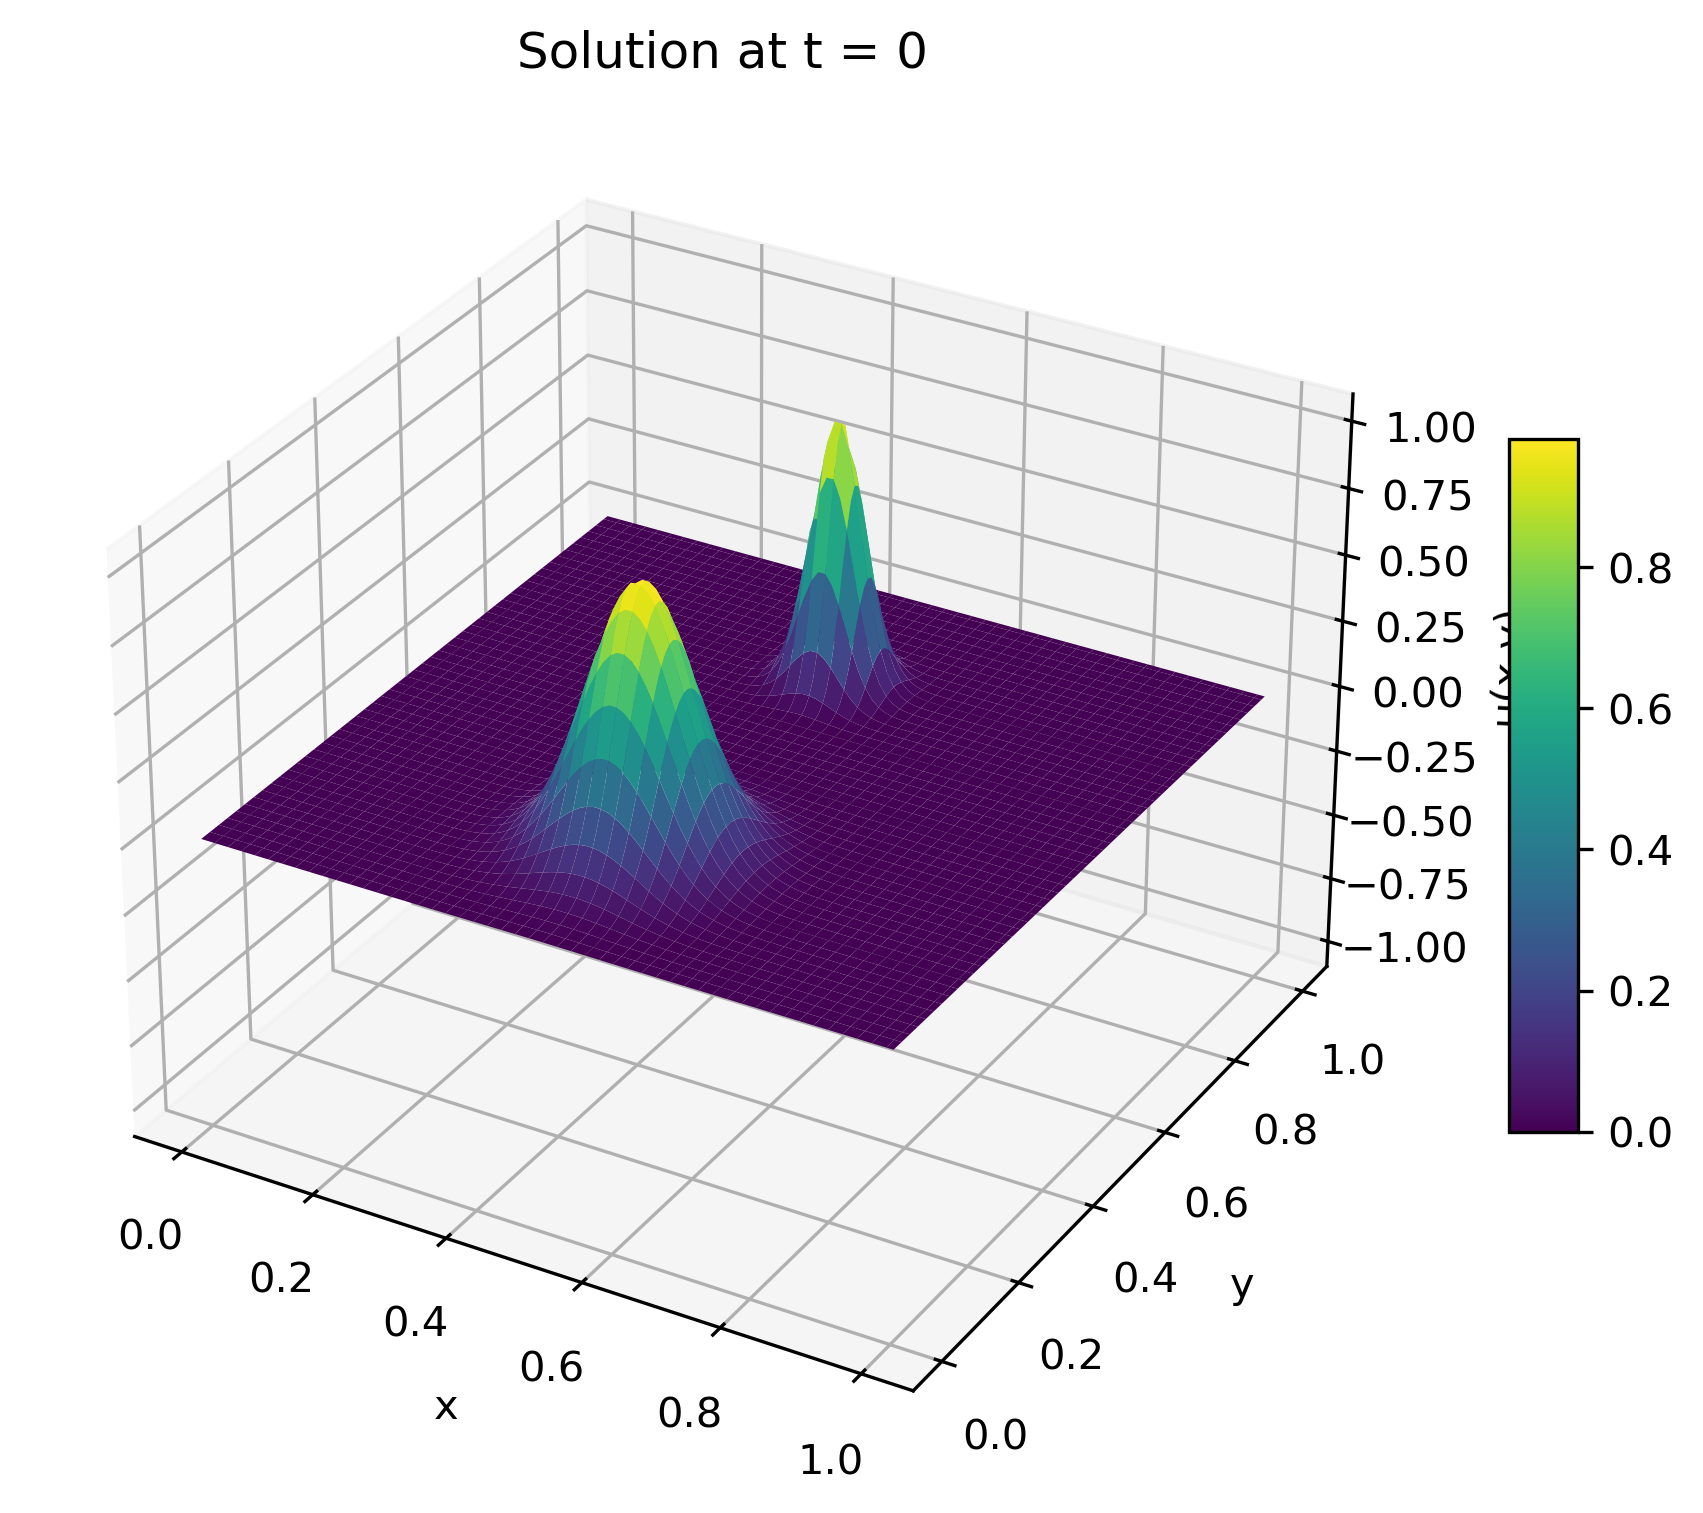
\includegraphics[width=\linewidth]{../plots/snapshot-0.00-complicated.png}
        \caption{$t = 0.00$}
    \end{subfigure}
    \hfill
        \begin{subfigure}{0.32\textwidth}
        \centering
        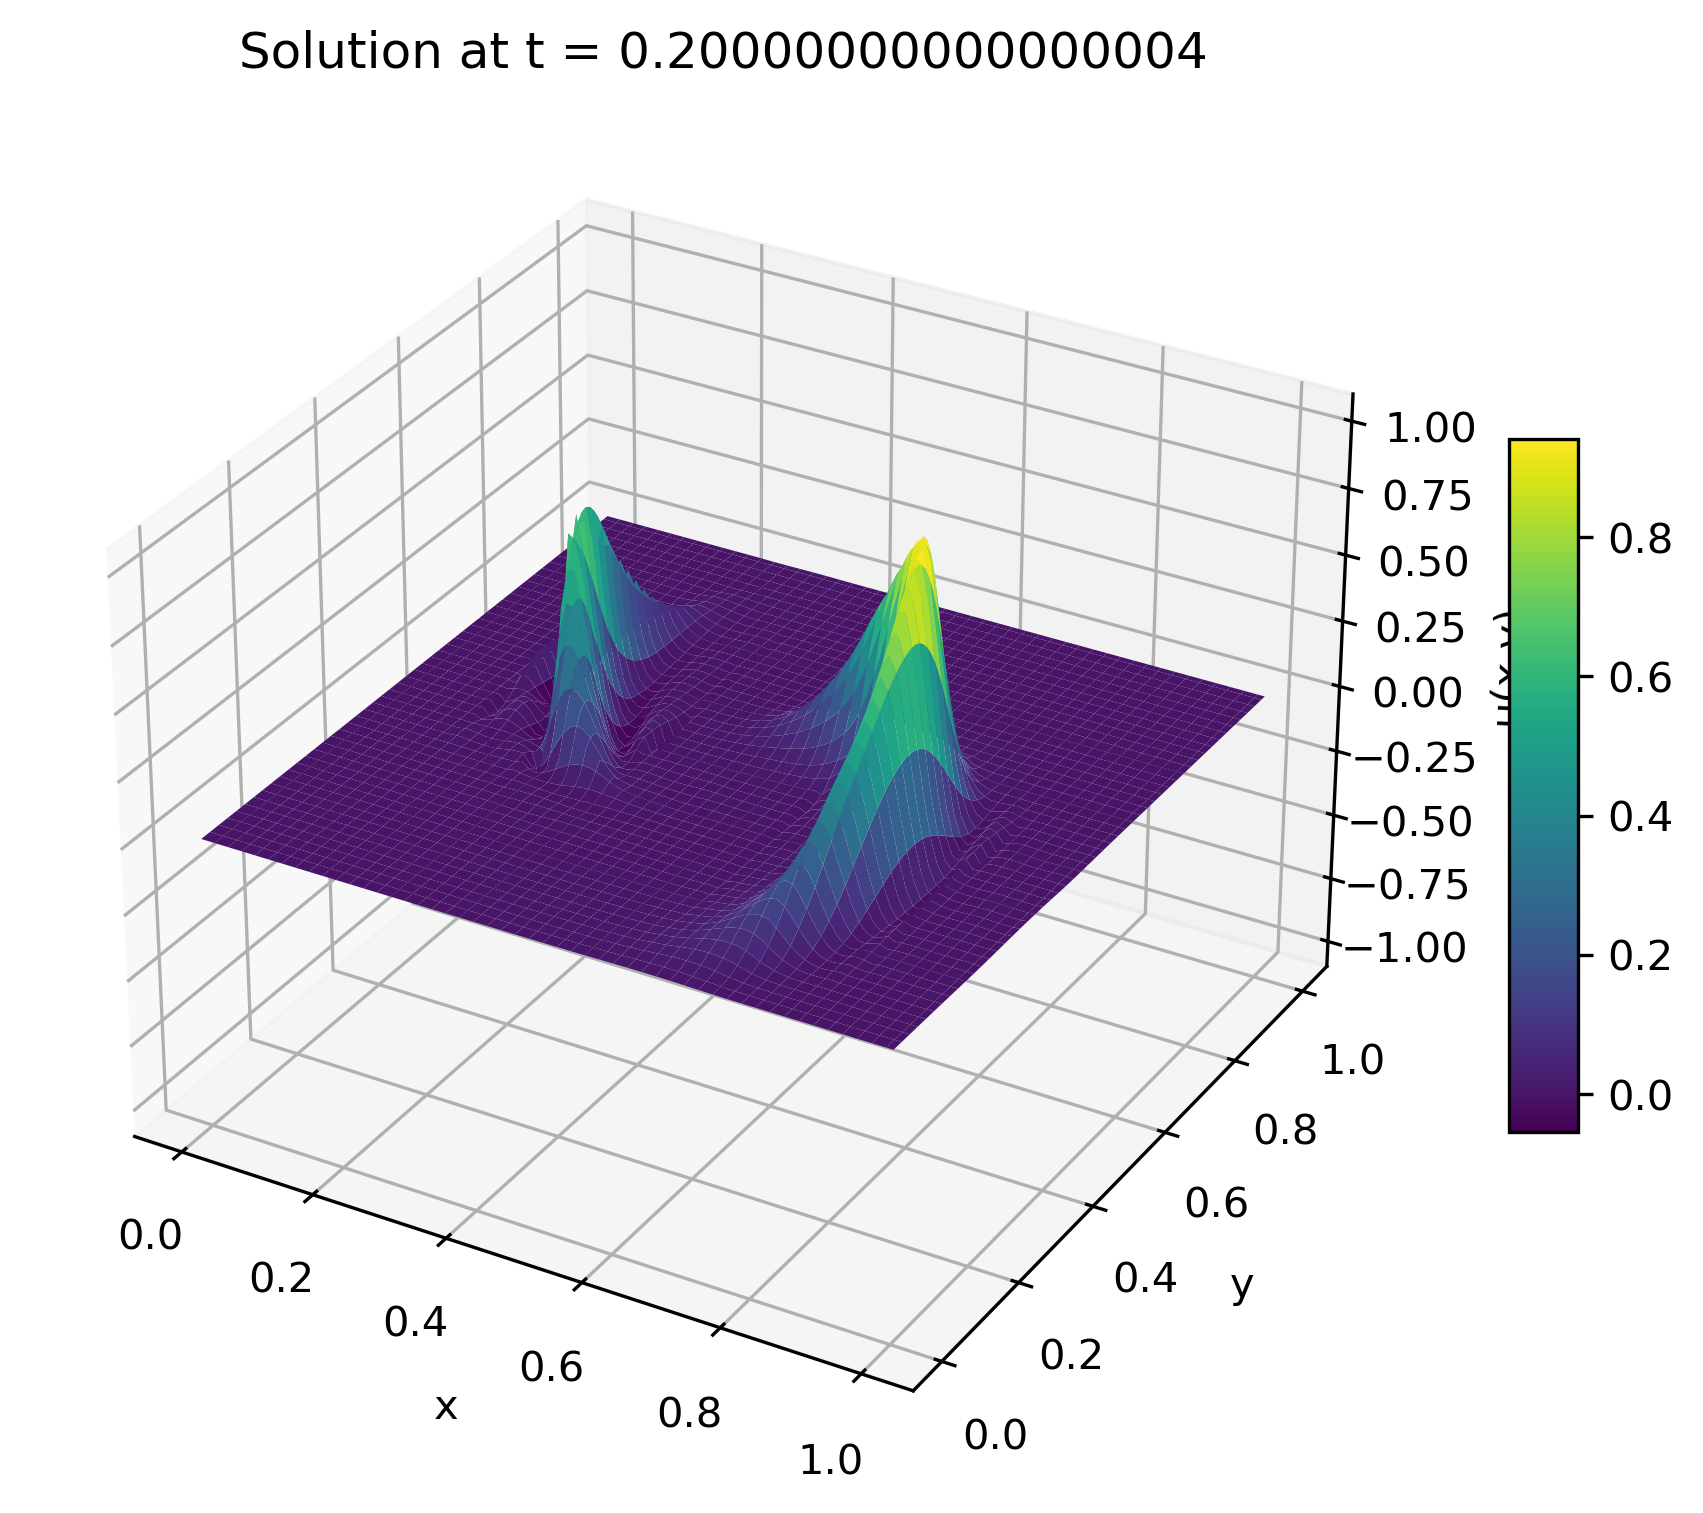
\includegraphics[width=\linewidth]{../plots/snapshot-0.20-complicated.png}
        \caption{$t = 0.20$}
    \end{subfigure}
    \hfill
    \begin{subfigure}{0.32\textwidth}
        \centering
        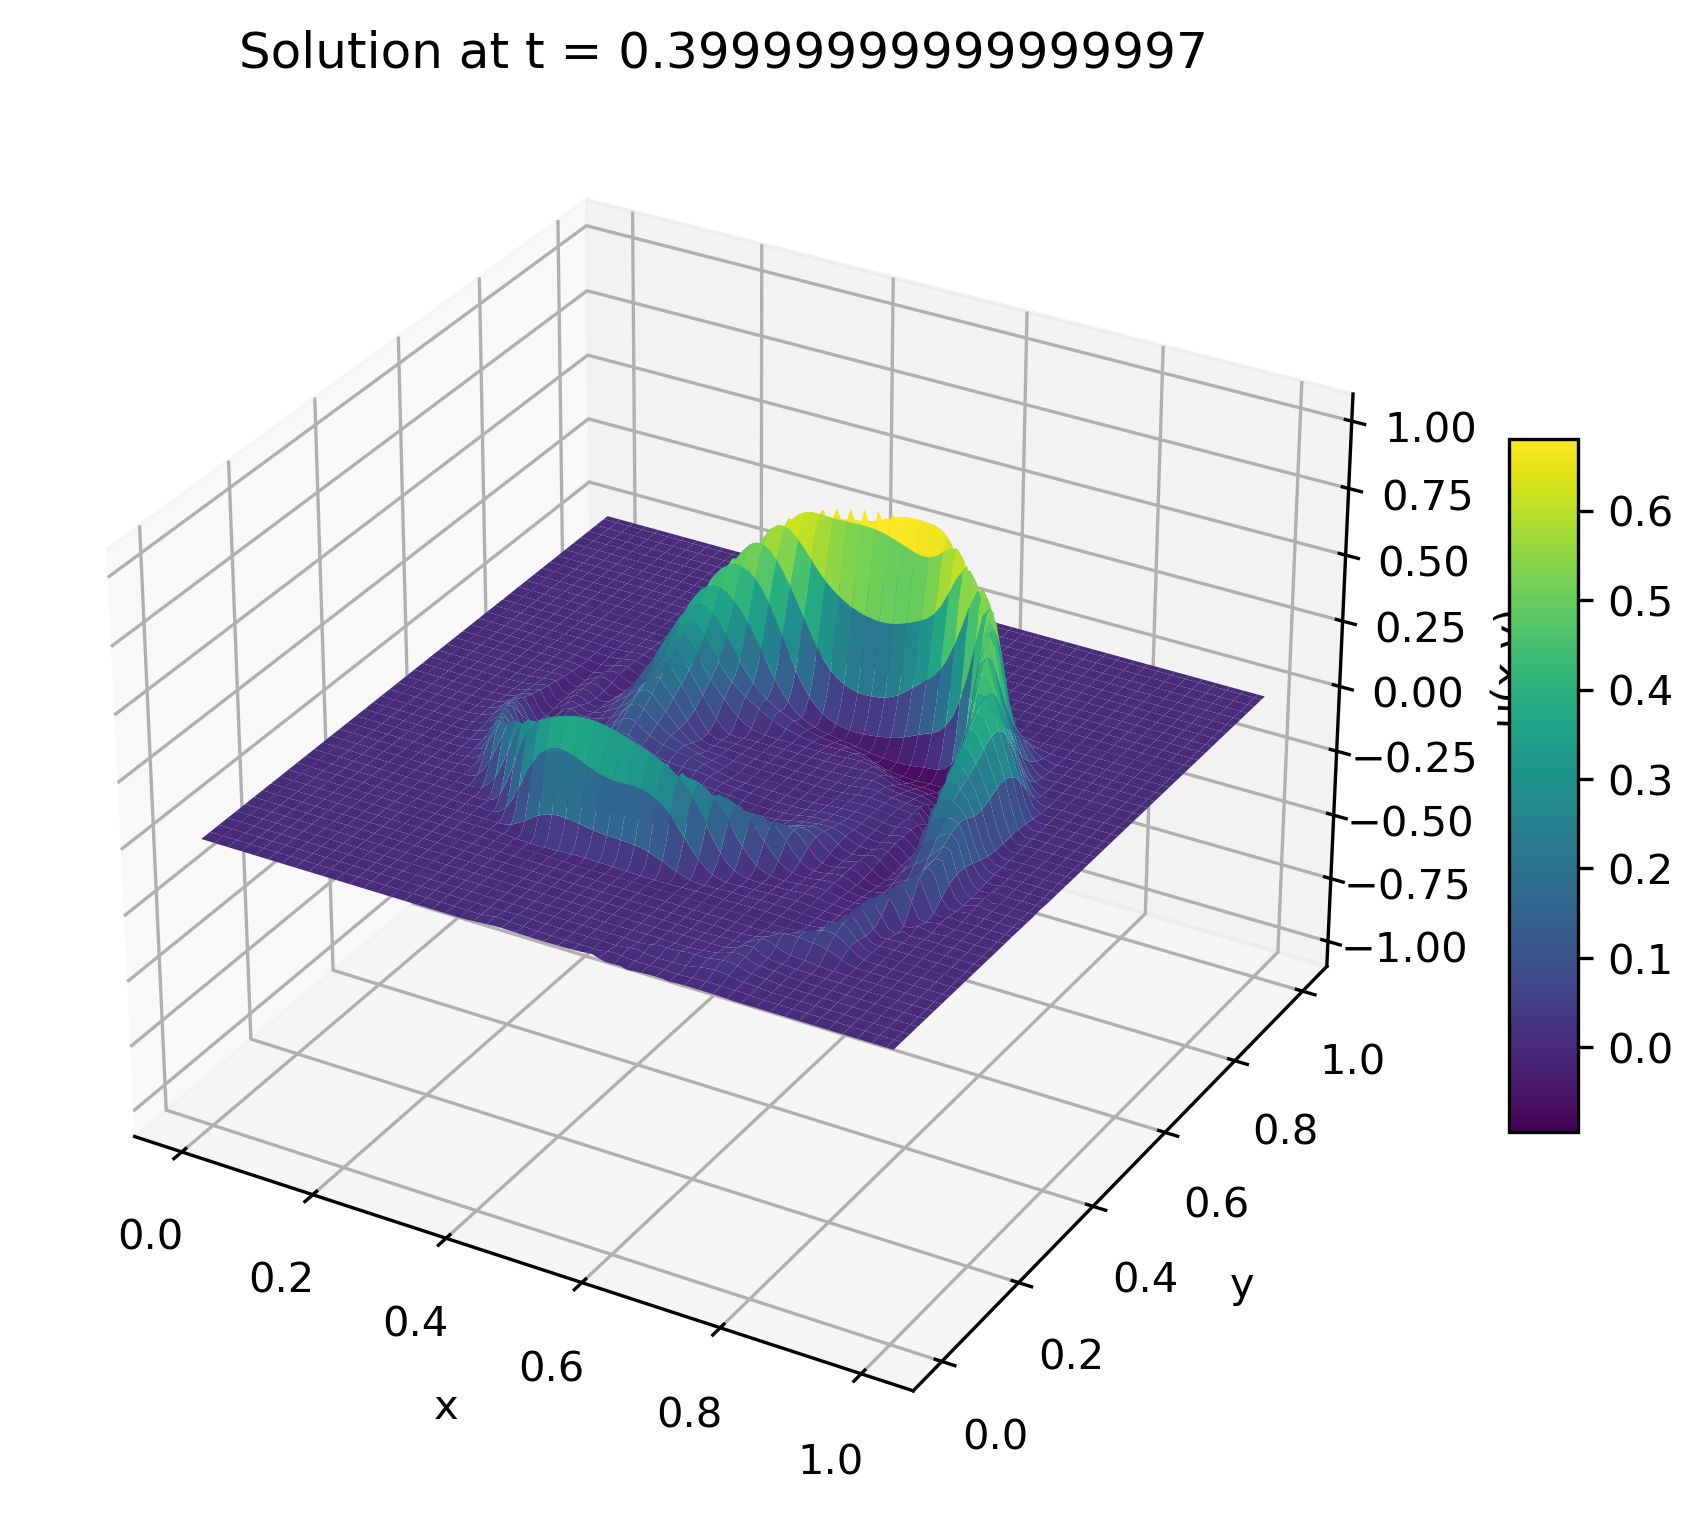
\includegraphics[width=\linewidth]{../plots/snapshot-0.40-complicated.png}
        \caption{$t = 0.40$}
    \end{subfigure}
    \hfill
    \begin{subfigure}{0.32\textwidth}
        \centering
        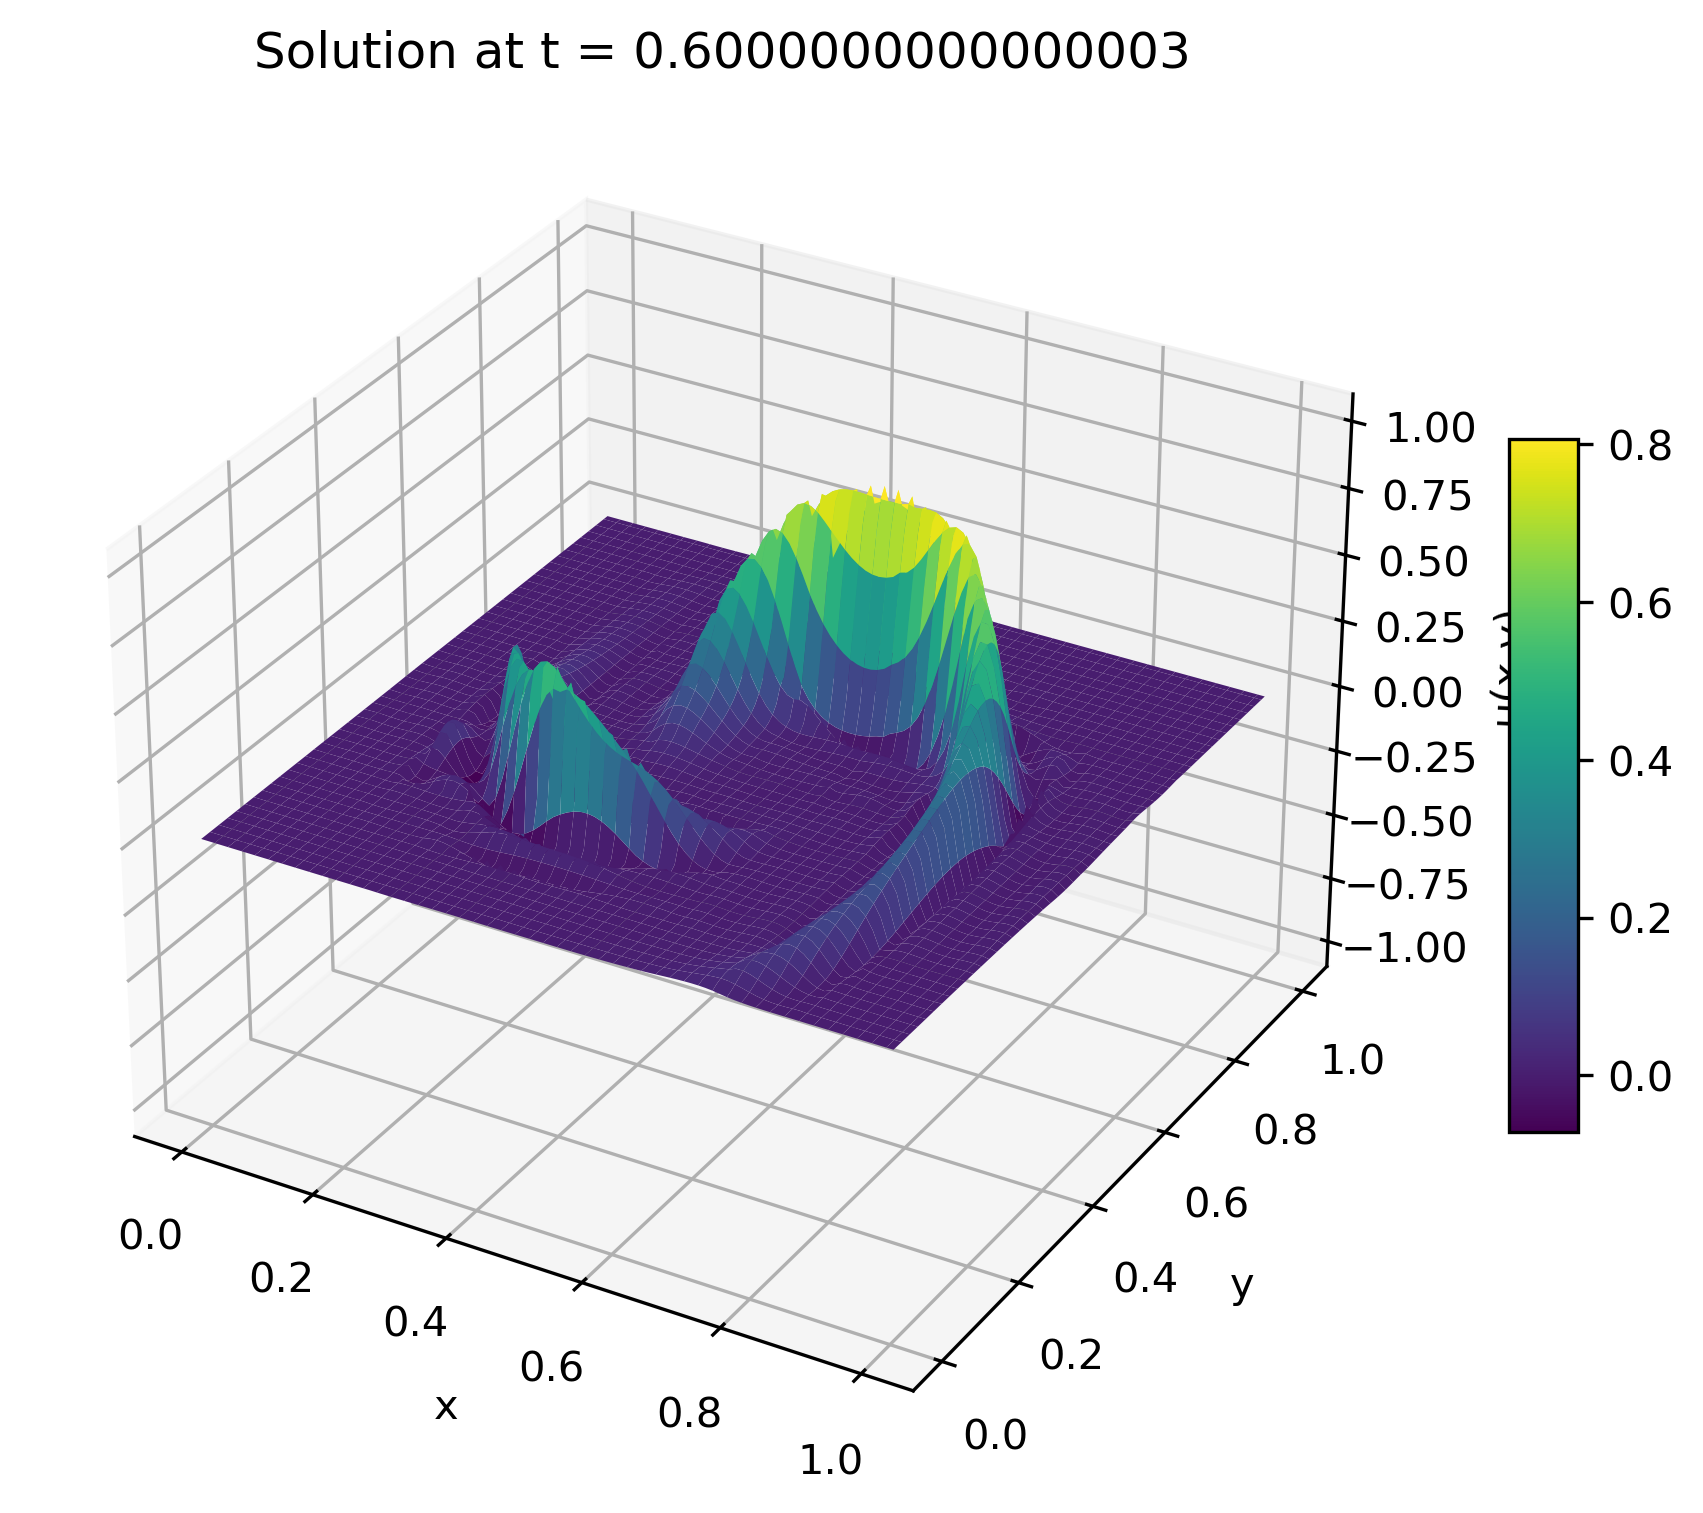
\includegraphics[width=\linewidth]{../plots/snapshot-0.60-complicated.png}
        \caption{$t = 0.60$}
    \end{subfigure}
    \hfill
    \begin{subfigure}{0.32\textwidth}
        \centering
        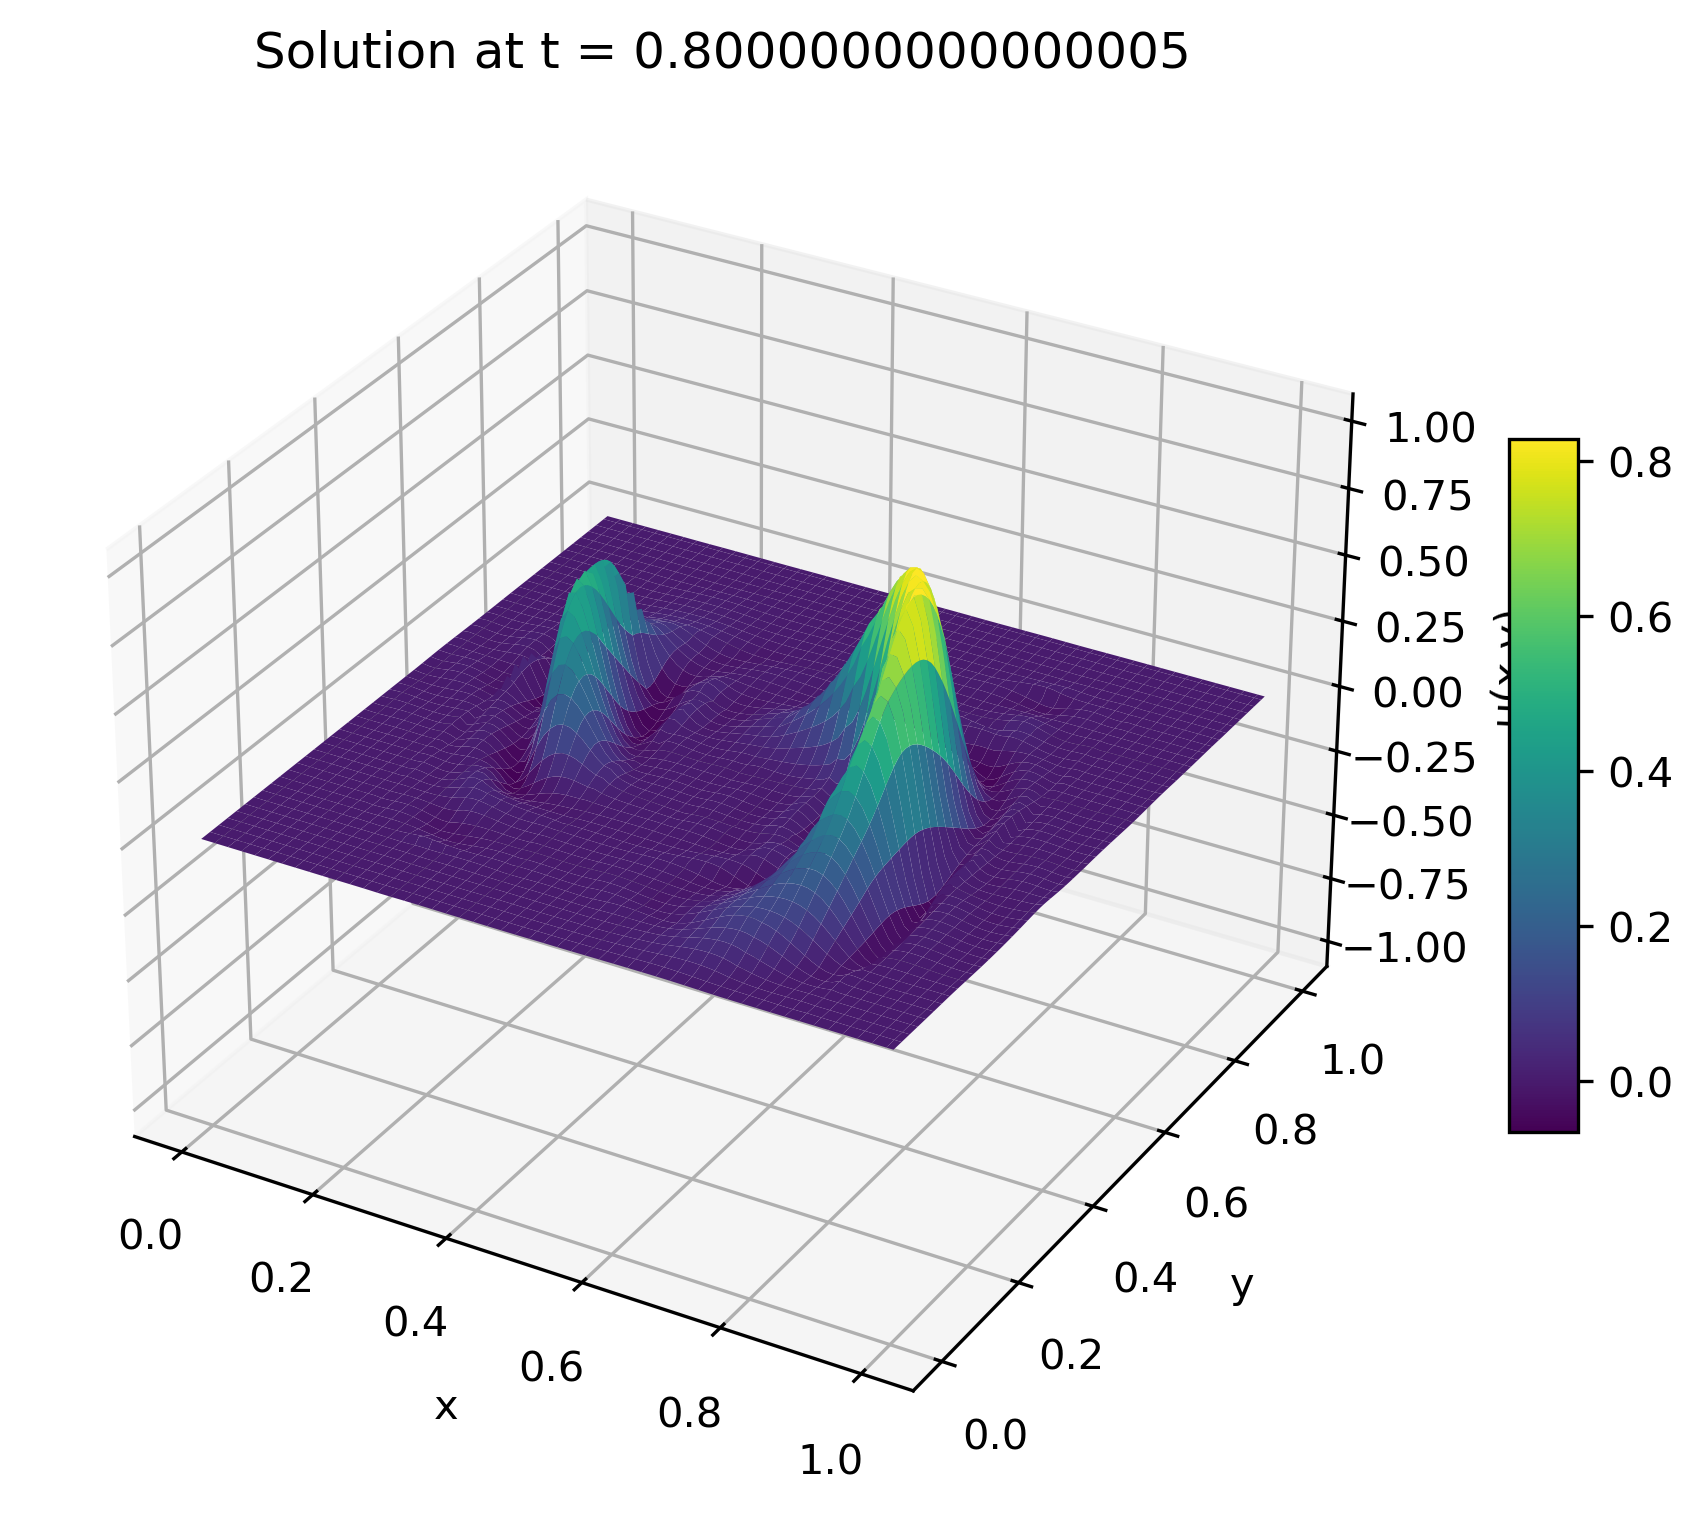
\includegraphics[width=\linewidth]{../plots/snapshot-0.80-complicated.png}
        \caption{$t = 0.80$}
    \end{subfigure}
    \hfill
    \begin{subfigure}{0.32\textwidth}
        \centering
        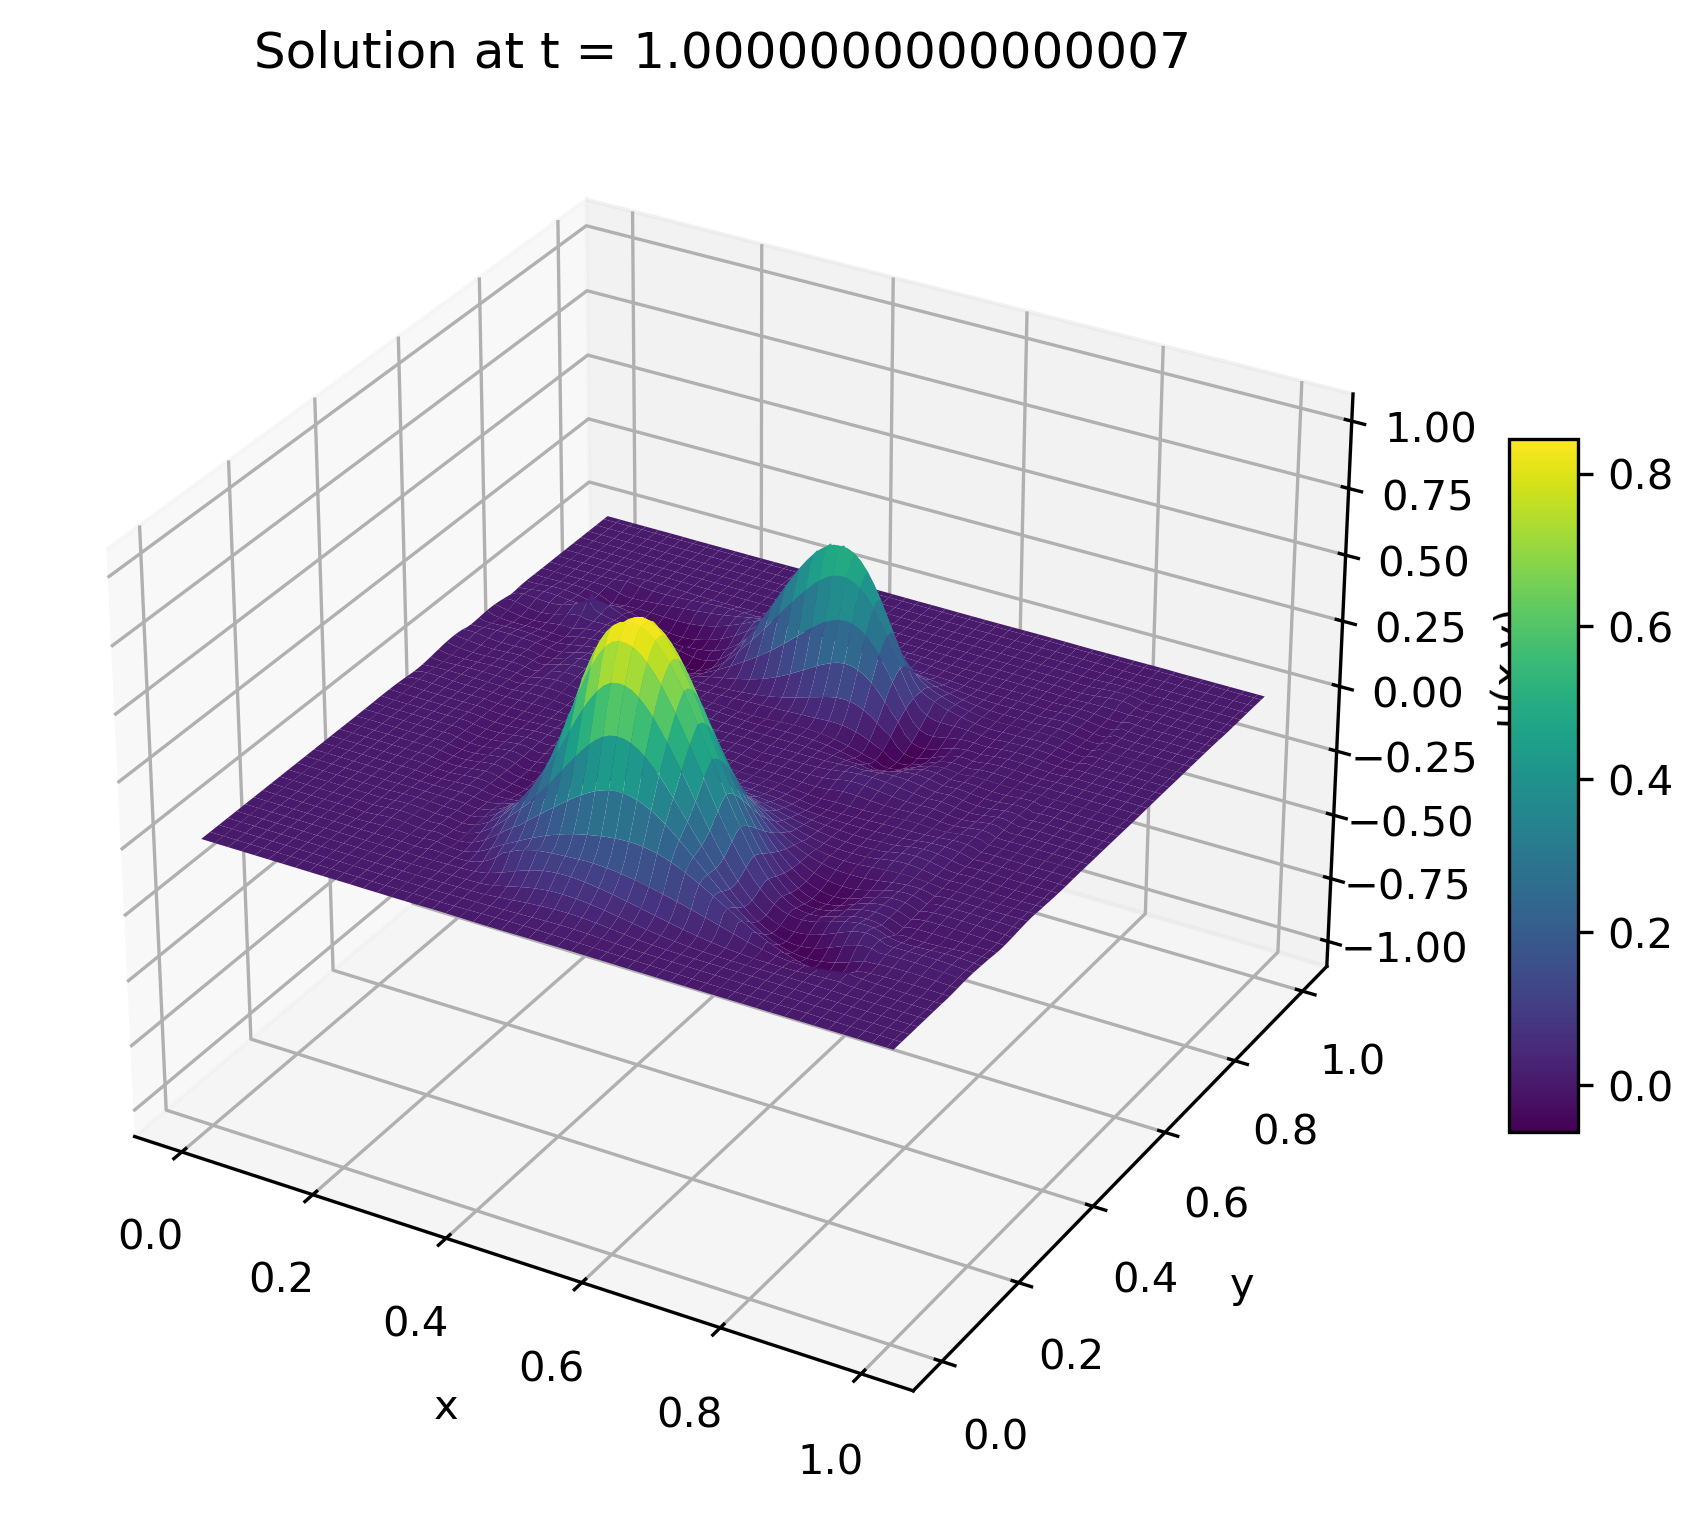
\includegraphics[width=\linewidth]{../plots/snapshot-1.00-complicated.png}
        \caption{$t = 1.00$}
    \end{subfigure}

    \caption{Snapshots of the approximate solution at selected times. $Nx = Ny = 32$, $p = 4$, $h = 0.01$, implicit RK4.}
    \label{fig:exact}    
\end{figure}

%%% Bibliography
\bibliographystyle{alpha}
\bibliography{references}
%%%

\end{document}
